The MC modelling of the inclusive $t\bar{t}$+jets background,
generated with \textsc{Powheg}+\textsc{Pythia8} and inclusive in up to six additional jets,
is known to exhibit residual mismodelling in regions with large jet multiplicity
and enhanced heavy-flavour content.
Since $t\bar{t}$+jets constitutes the dominant background in the signal-enriched regions of this analysis,
data-driven corrections are derived and applied prior to the signal extraction fit.

Two largely independent sources of mismodelling are observed:
an underestimation of the $t\bar{t}$ production rate in association
with heavy-flavour jets ($t\bar{t}$+HF),
and imperfect modelling of the jet multiplicity spectrum and
correlated kinematic properties of additional jets.
These effects are addressed through a two-step correction strategy,
consisting of a flavour-dependent normalisation rescaling
and a multivariate kinematic reweighting.

\subsection{Flavour-dependent normalisation rescaling}
\label{sec:hf_rew_thesis}

The first source of mismodelling arises from the flavour composition
of the $t\bar{t}$+jets sample.
Several ATLAS measurements in final states with high jet multiplicity
have reported discrepancies between data and simulation
in the relative contributions of $t\bar{t}$ events with different
additional jet flavours, in particular in the heavy-flavour components.
In this analysis, the $t\bar{t}$+jets sample is categorised according to the flavour of additional jets into
$t\bar{t}+\mathrm{light}$ (TTL),
$t\bar{t}+\ge1c$ (TTC), and
$t\bar{t}+\ge1b$ (TTB),
dedicated scale factors are extracted from data to correct
their relative normalisations and therefore the overall flavour composition
of the $t\bar{t}$+jets background.

The scale factors are obtained from a background-dominated likelihood fit using the sum of the pseudo-continuous $b$-tagging discriminants of the third and fourth jets ranked by the DL1r score,
$\mathrm{pcb}(j_3)+\mathrm{pcb}(j_4)$,
which provides strong discrimination between TTL, TTC and TTB components.
The fit is performed simultaneously in the 1L and 2LOS channels using regions with exactly two, exactly three, and at least four $b$-tagged jets.
To minimise signal bias, the fit regions are chosen such that the signal contamination is negligible for all signal hypotheses. 
The signal-to-background ratios are summarised in Table~\ref{tab:sigContam_HFCorrRegion}.

\begin{table}[htbp]
  \centering
  \def\arraystretch{1.15}
  \begin{tabular}{c|cc}
    \toprule
      & 1L ($=7j$) & 2LOS ($=5j$) \\
    \midrule
    $=2b$    & $<0.1\%$ & $<0.1\%$ \\
    $=3b$    & $<0.1\%$ & $<0.1\%$ \\
    $\ge4b$  & $0.2\%$  & $0.1\%$ \\
    \bottomrule
  \end{tabular}
  \caption{Signal-to-background ratio in the regions used to derive the flavour rescaling factors (illustrated for the BSMtttt $m=700$~GeV hypothesis), prior to applying any data-driven corrections.}
  \label{tab:sigContam_HFCorrRegion}
\end{table}

In the fit, the normalisations of TTL, TTC and TTB are free to float.
The TTL normalisation is treated independently in the 1L and 2LOS channels to account for acceptance differences between channels, while TTC and TTB are constrained to be common.
Nuisance parameters associated with $b$-tagging uncertainties (Section~\ref{b-tagging_uncertianties}) and the normalisation uncertainties of sub-dominant backgrounds are included, as they impact the flavour composition in the fit regions.

The fit significantly improves the agreement between data and simulation
in the $\mathrm{pcb}(j_3)+\mathrm{pcb}(j_4)$ distributions
as illustrated in Figures~\ref{fig:1L_pcb34_PrePost_thesis} and
\ref{fig:2LOS_pcb34_PrePost_thesis},
with fitted scale factors consistent with values reported in
ATLAS measurements targeting similar phase space~\cite{HIGG-2017-03}.
The fitted scale factors for the nominal and alternative $t\bar{t}$+jets samples are summarised in Table~\ref{tab:HF_results_thesis}.

% --- keep your existing plots but rename labels cleanly ---
\begin{figure}[htbp]
  \centering
  \subfloat[1L, $=7j$, $=2b$]{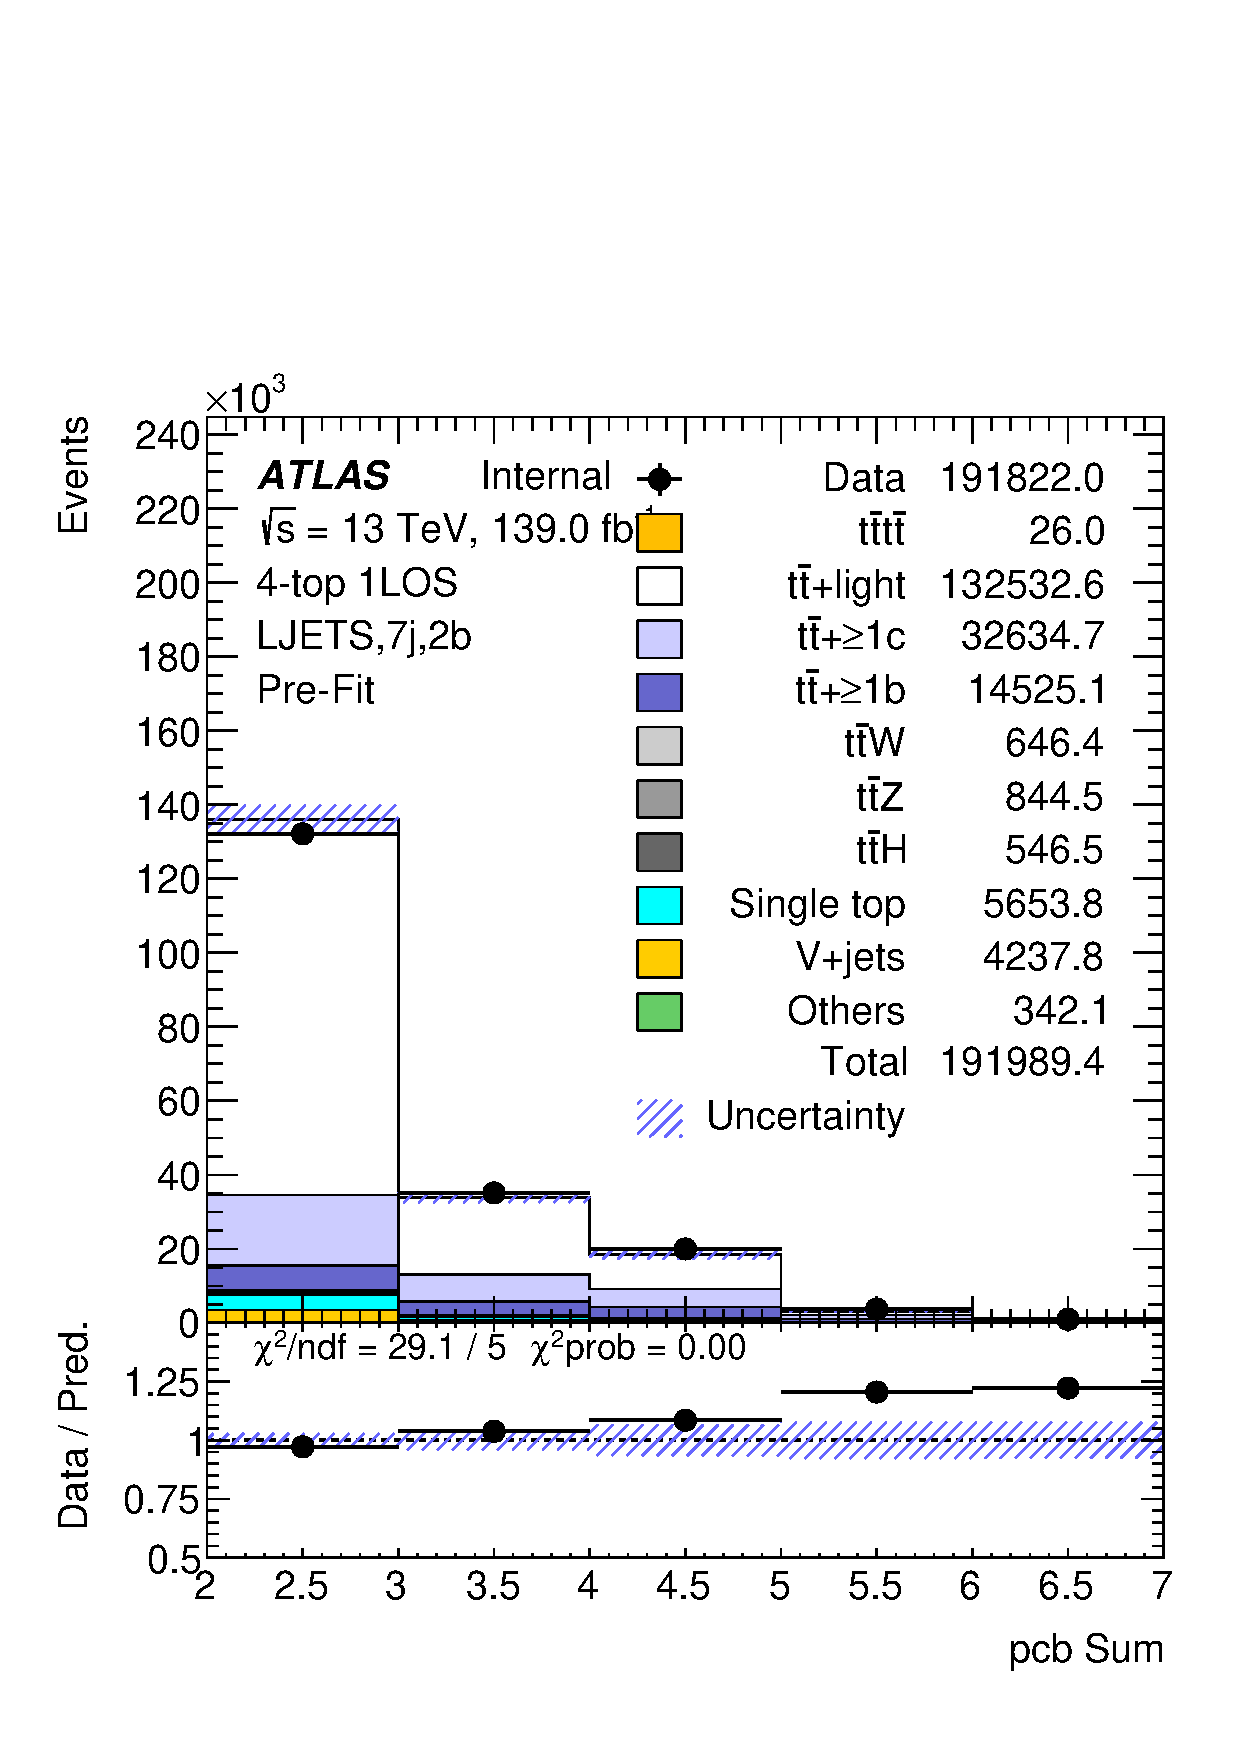
\includegraphics[height=0.28\textheight]{figures/pcbSum34_ljets_7j2b_preFit.pdf}}
  \subfloat[1L, $=7j$, $=2b$]{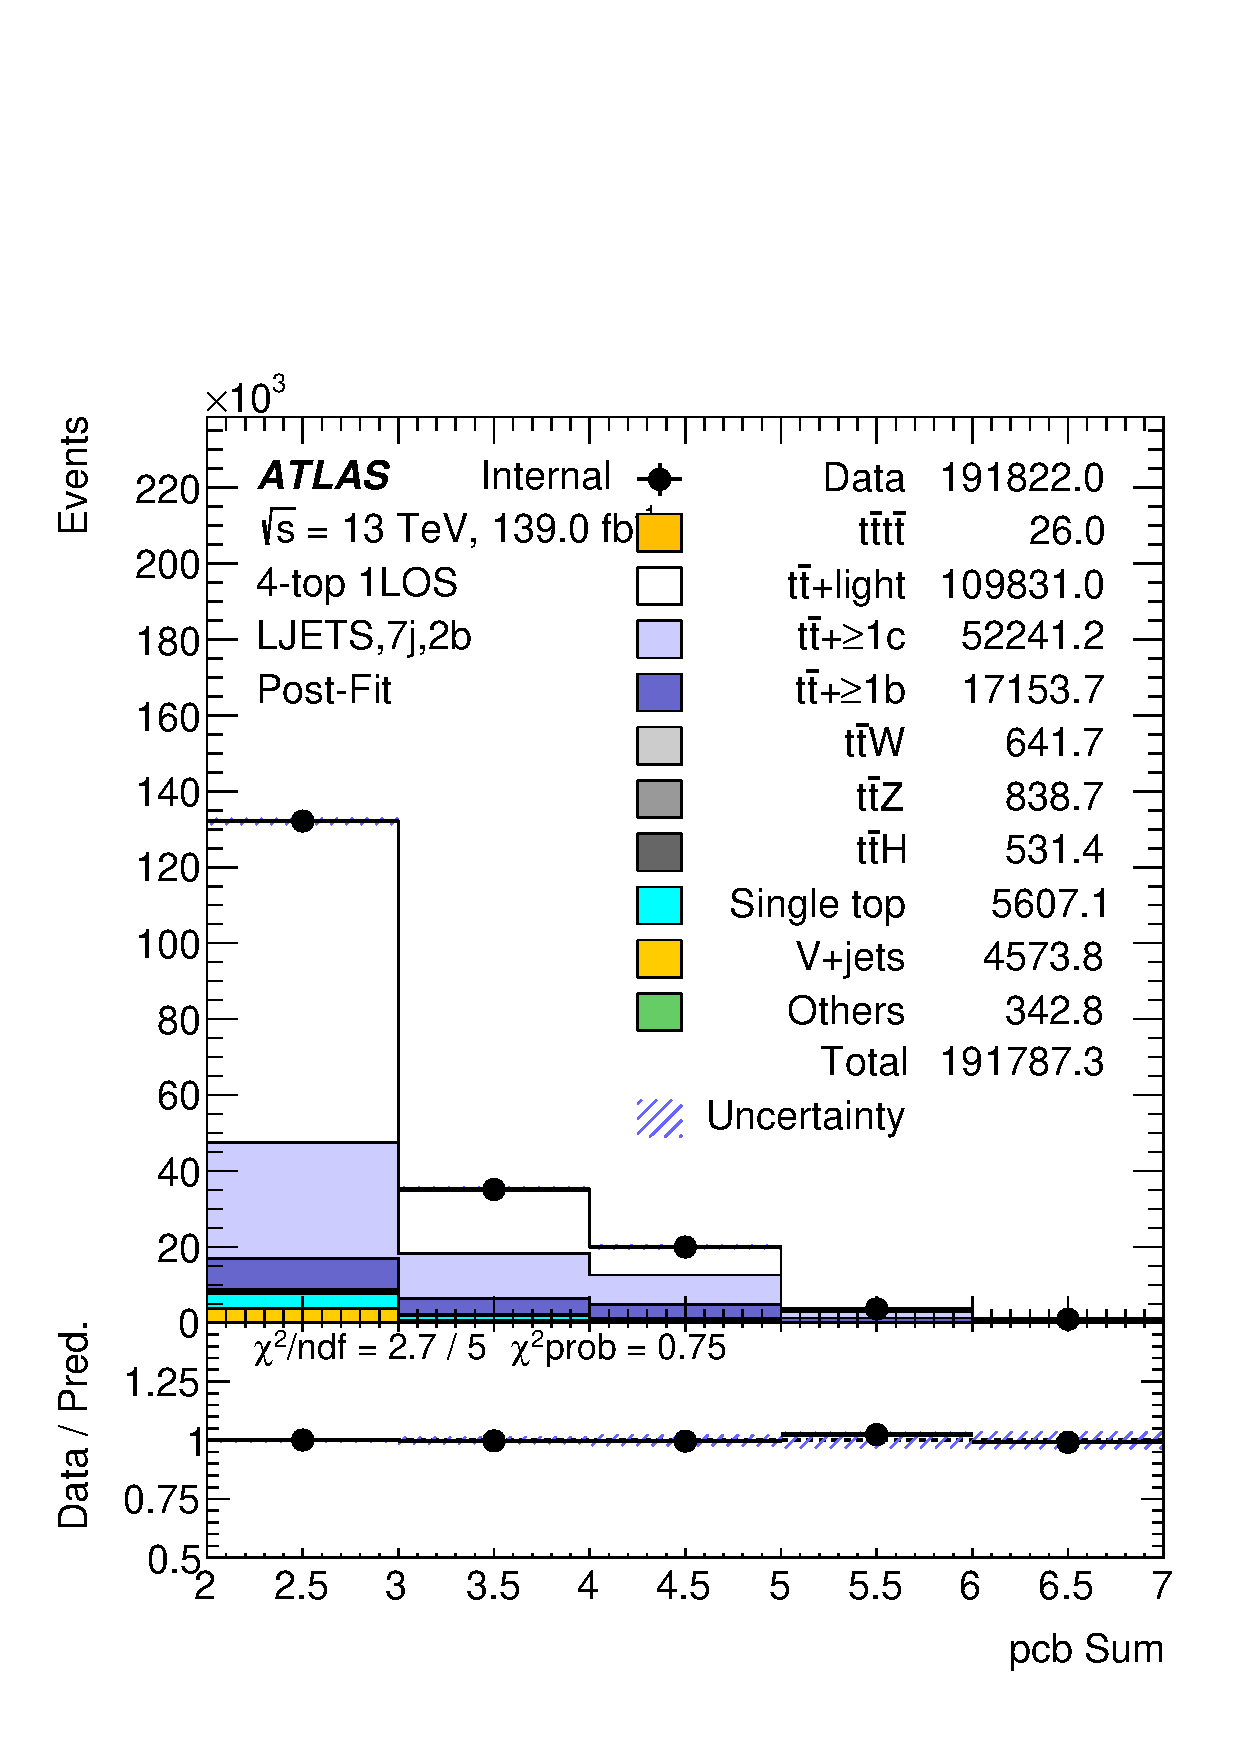
\includegraphics[height=0.28\textheight]{figures/pcbSum34_ljets_7j2b_postFit.pdf}}\\
  \subfloat[1L, $=7j$, $=3b$]{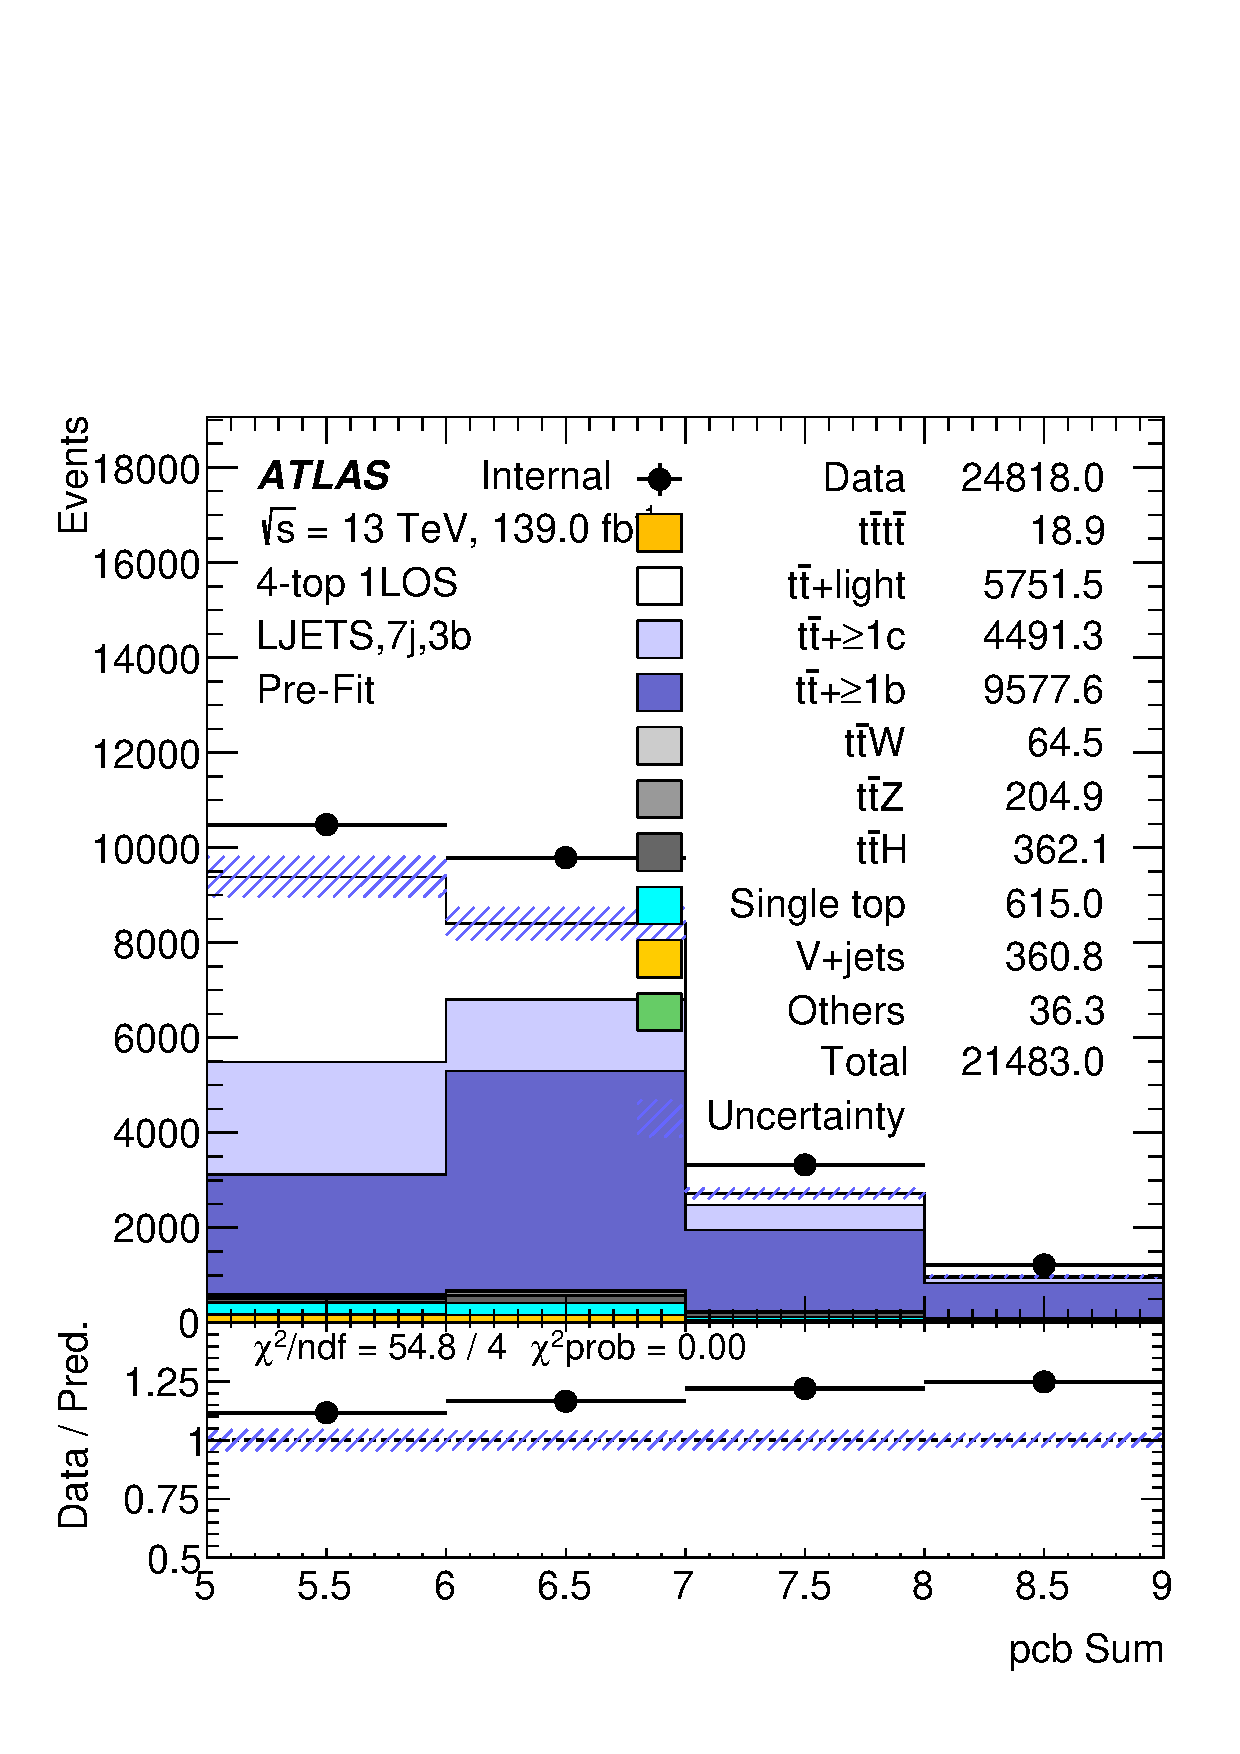
\includegraphics[height=0.28\textheight]{figures/pcbSum34_ljets_7j3b_preFit.pdf}}
  \subfloat[1L, $=7j$, $=3b$]{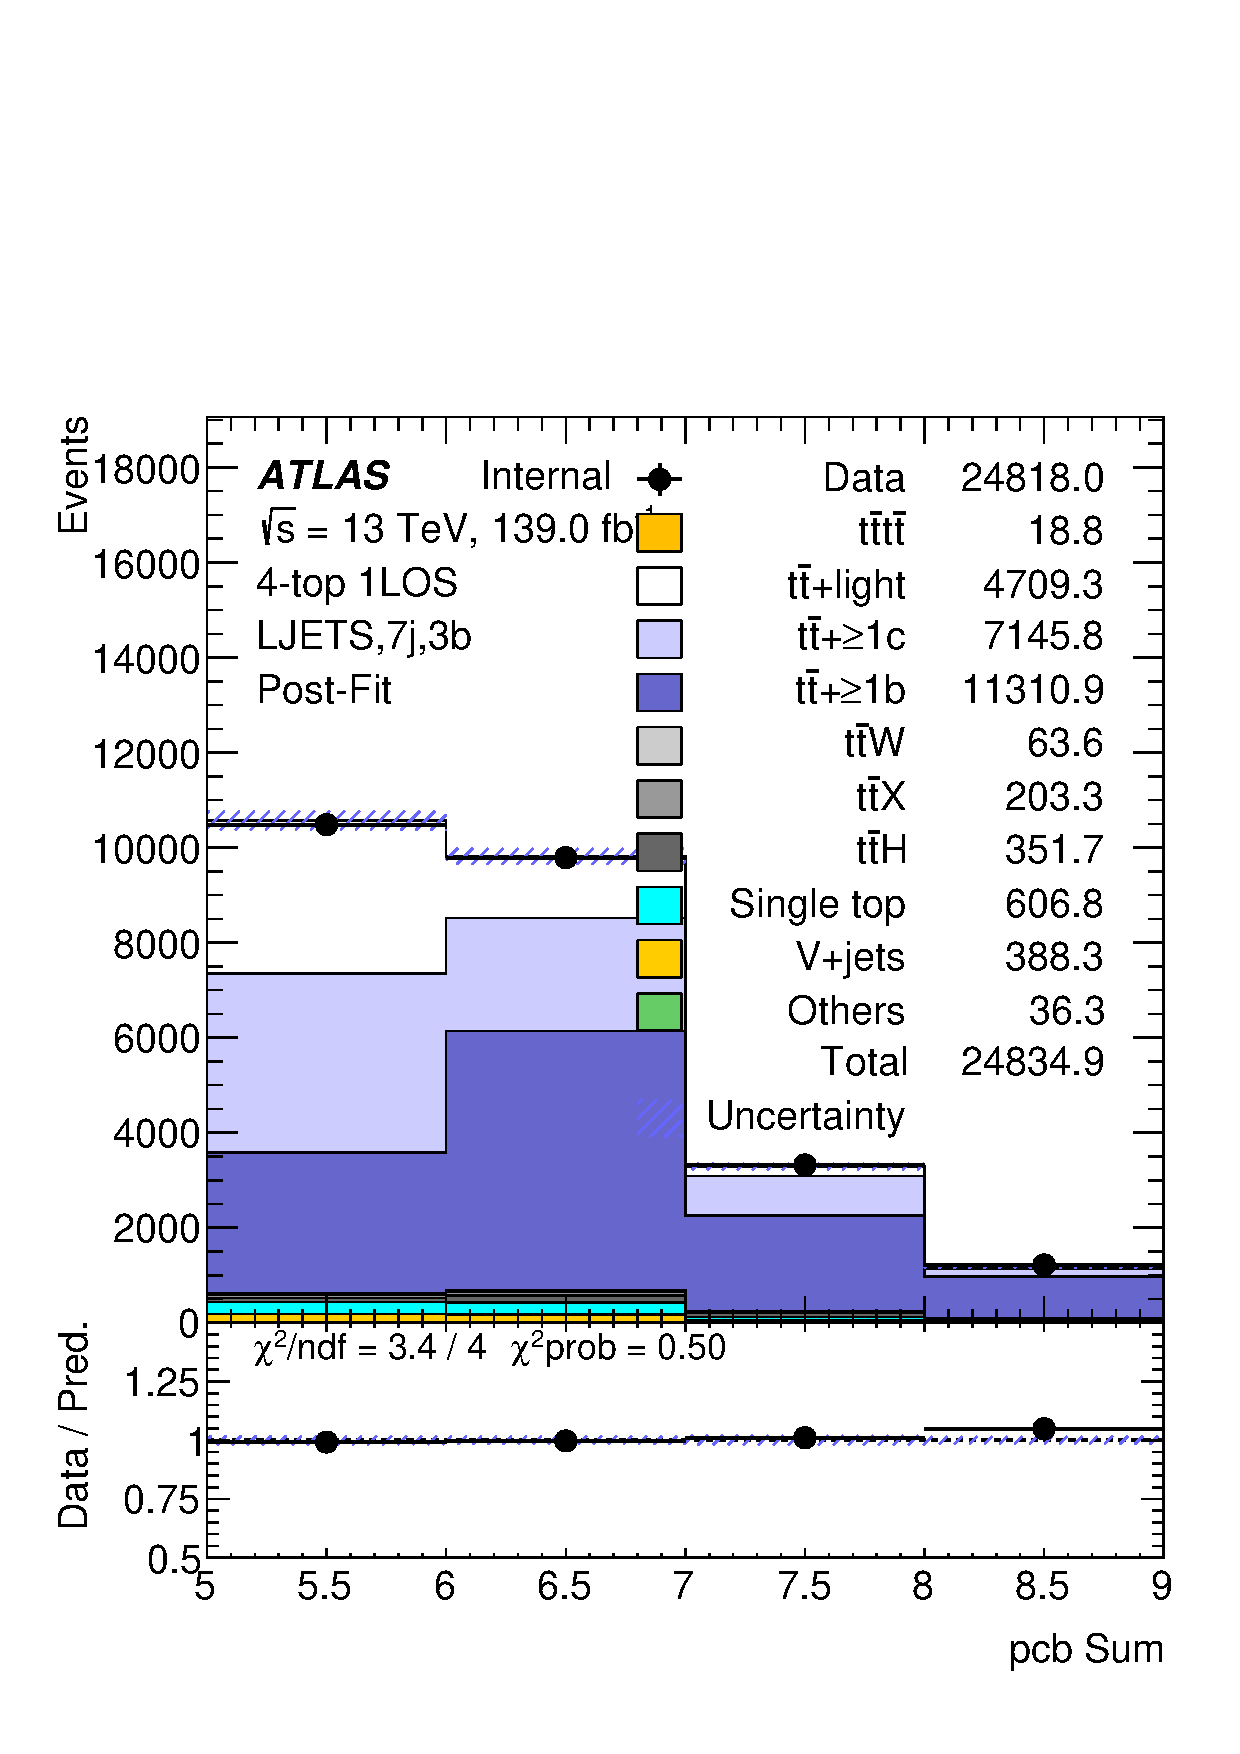
\includegraphics[height=0.28\textheight]{figures/pcbSum34_ljets_7j3b_postFit.pdf}}\\
  \subfloat[1L, $=7j$, $\ge4b$]{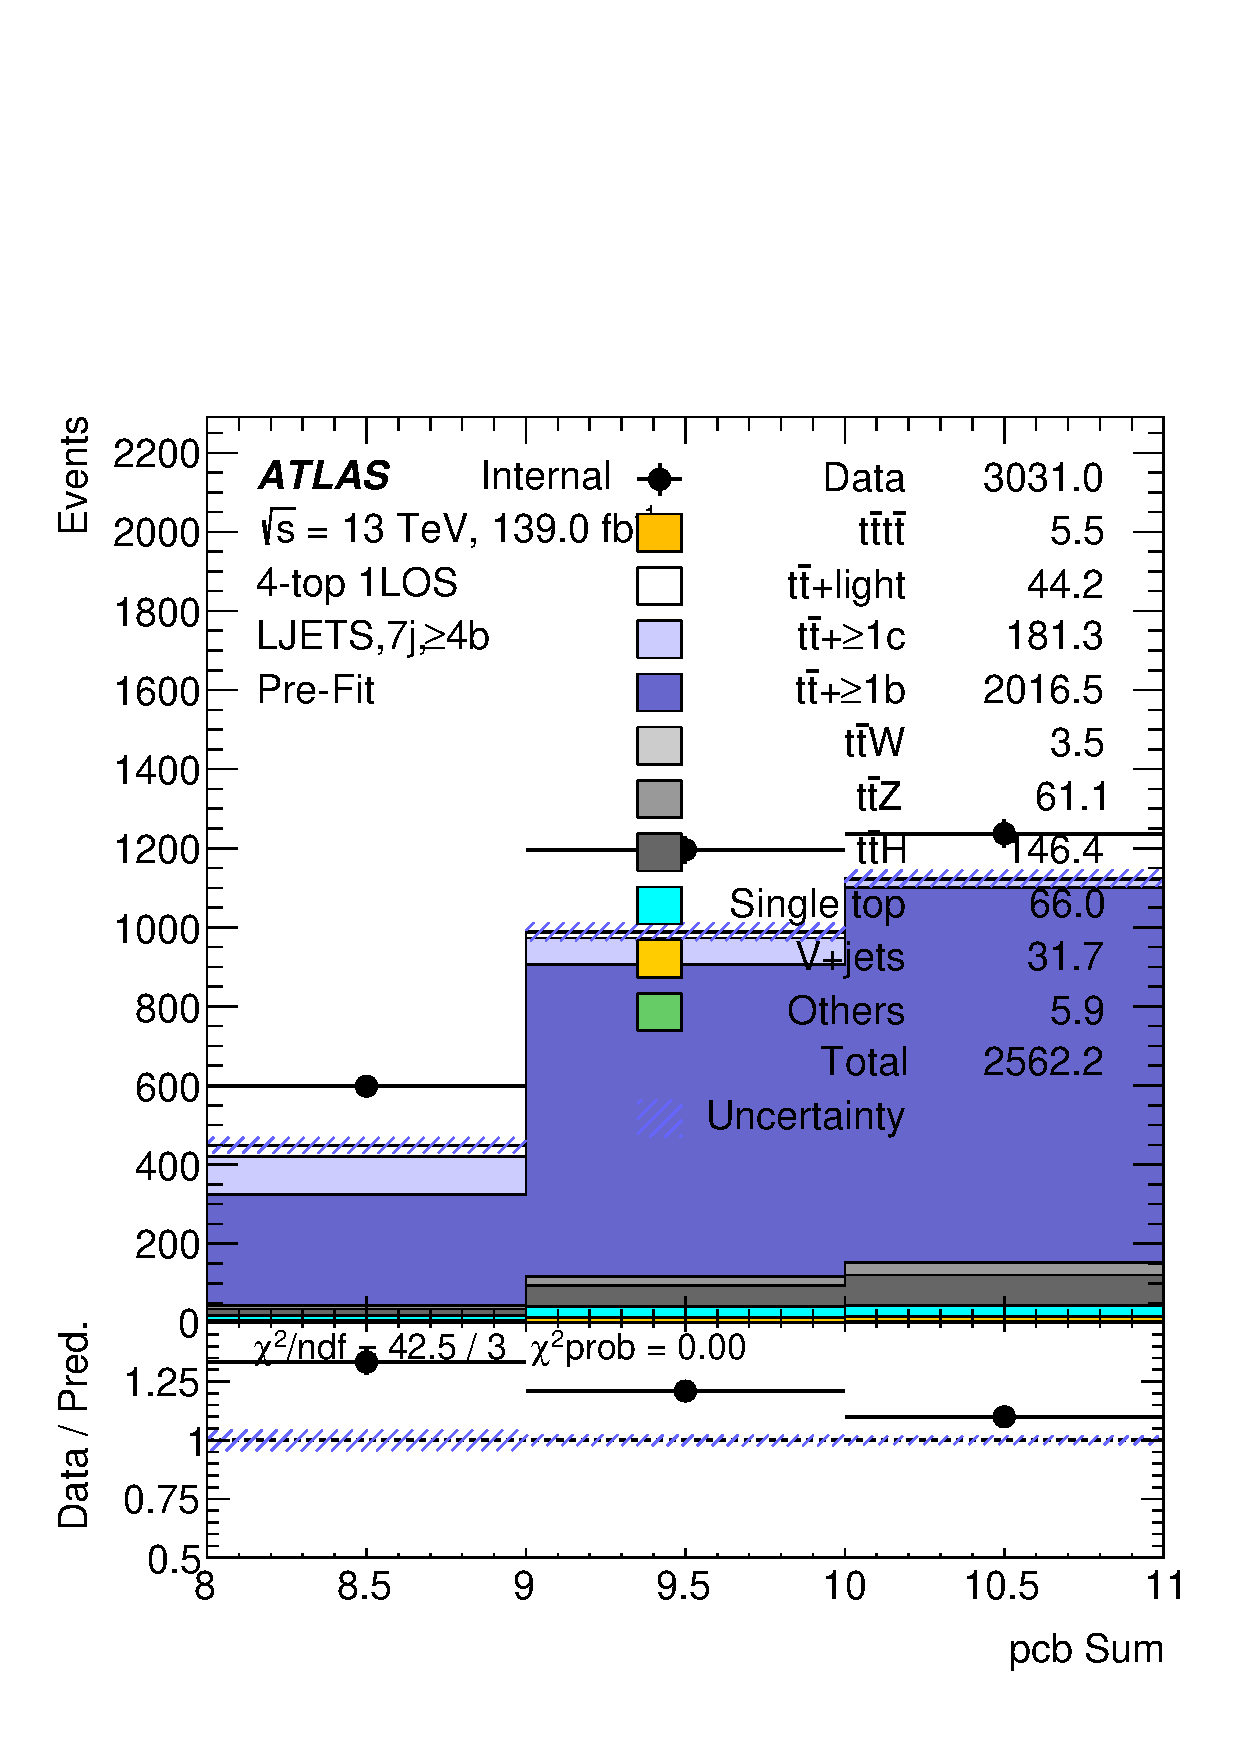
\includegraphics[height=0.28\textheight]{figures/pcbSum34_ljets_7jge4b_preFit.pdf}}
  \subfloat[1L, $=7j$, $\ge4b$]{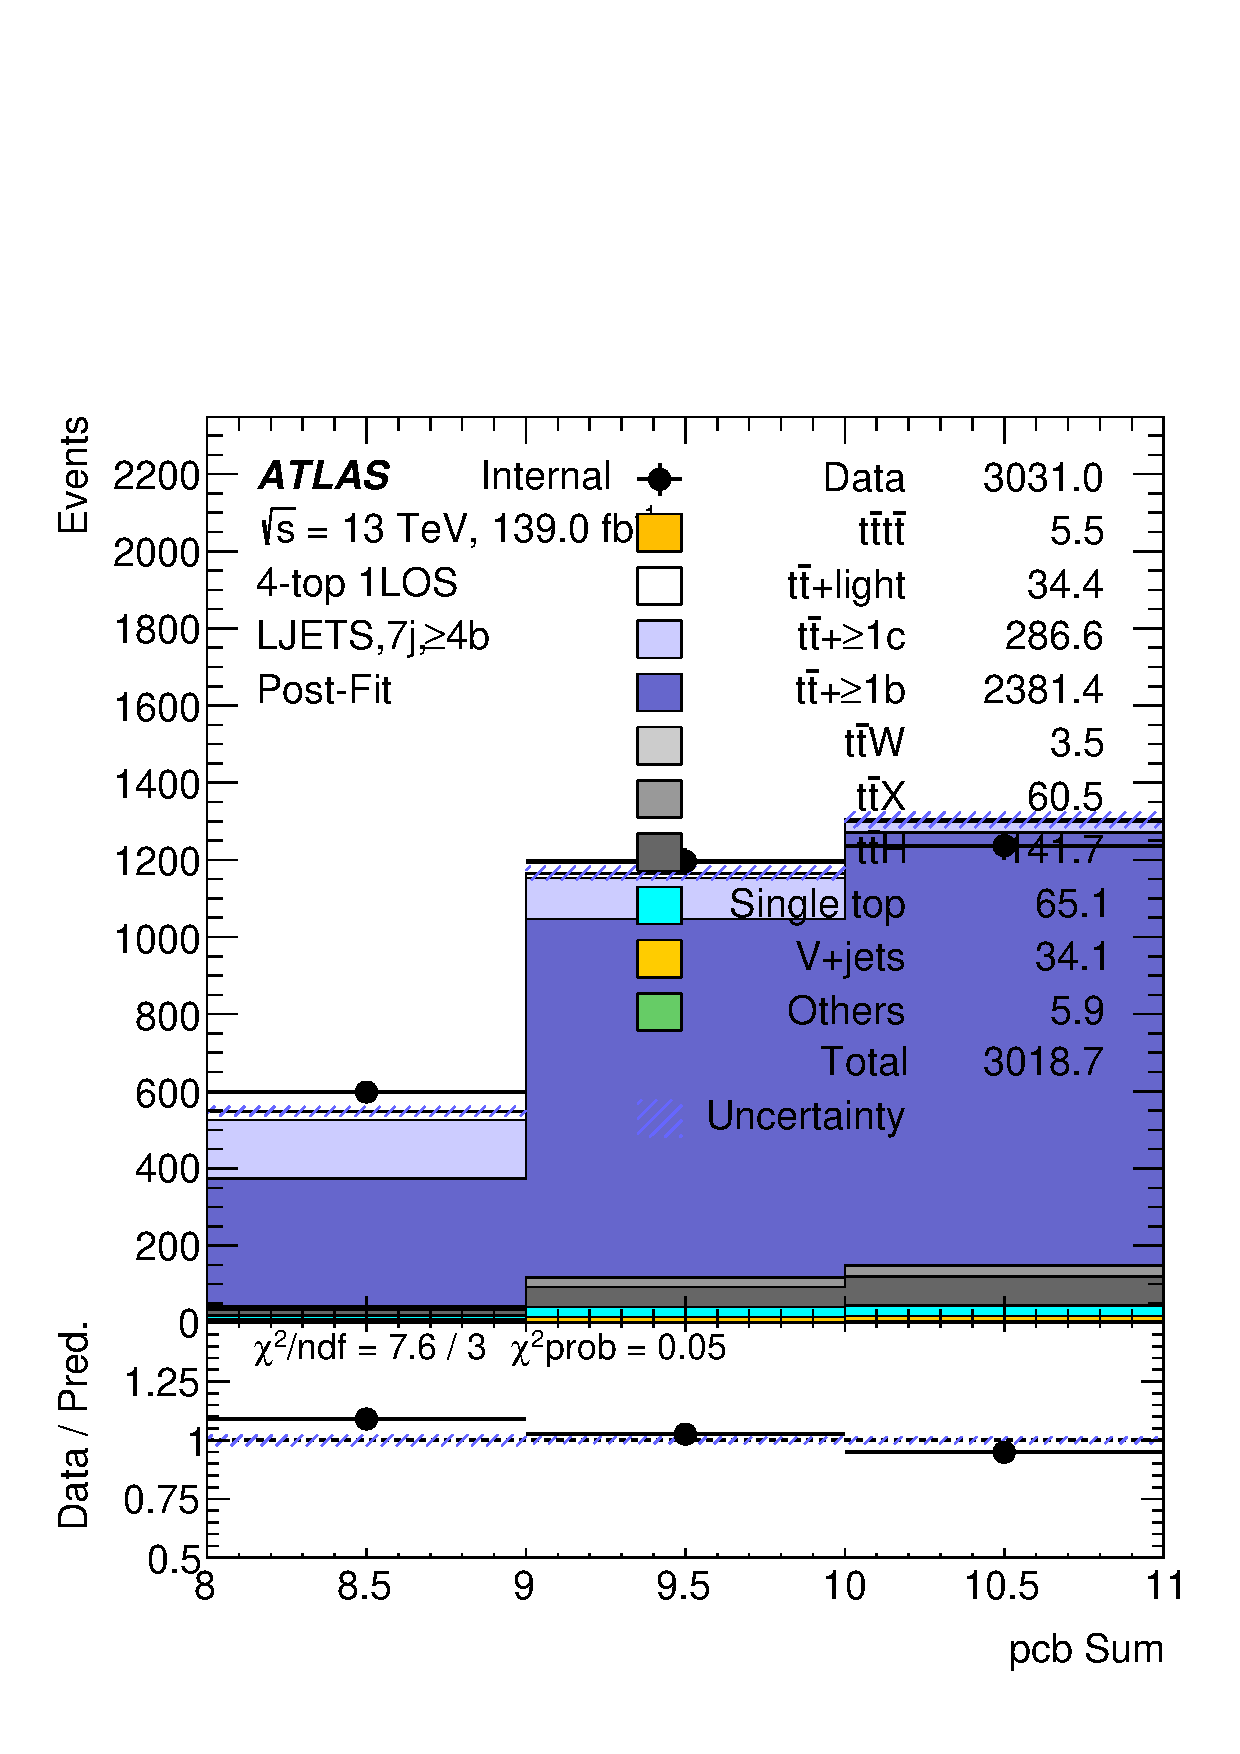
\includegraphics[height=0.28\textheight]{figures/pcbSum34_ljets_7jge4b_postFit.pdf}}
  \caption{Distributions of $\mathrm{pcb}(j_3)+\mathrm{pcb}(j_4)$ in the 1L flavour fit regions before (left) and after (right) the fit.}
  \label{fig:1L_pcb34_PrePost_thesis}
\end{figure}

\begin{figure}[htbp]
  \centering
  \subfloat[2LOS, $=5j$, $=2b$]{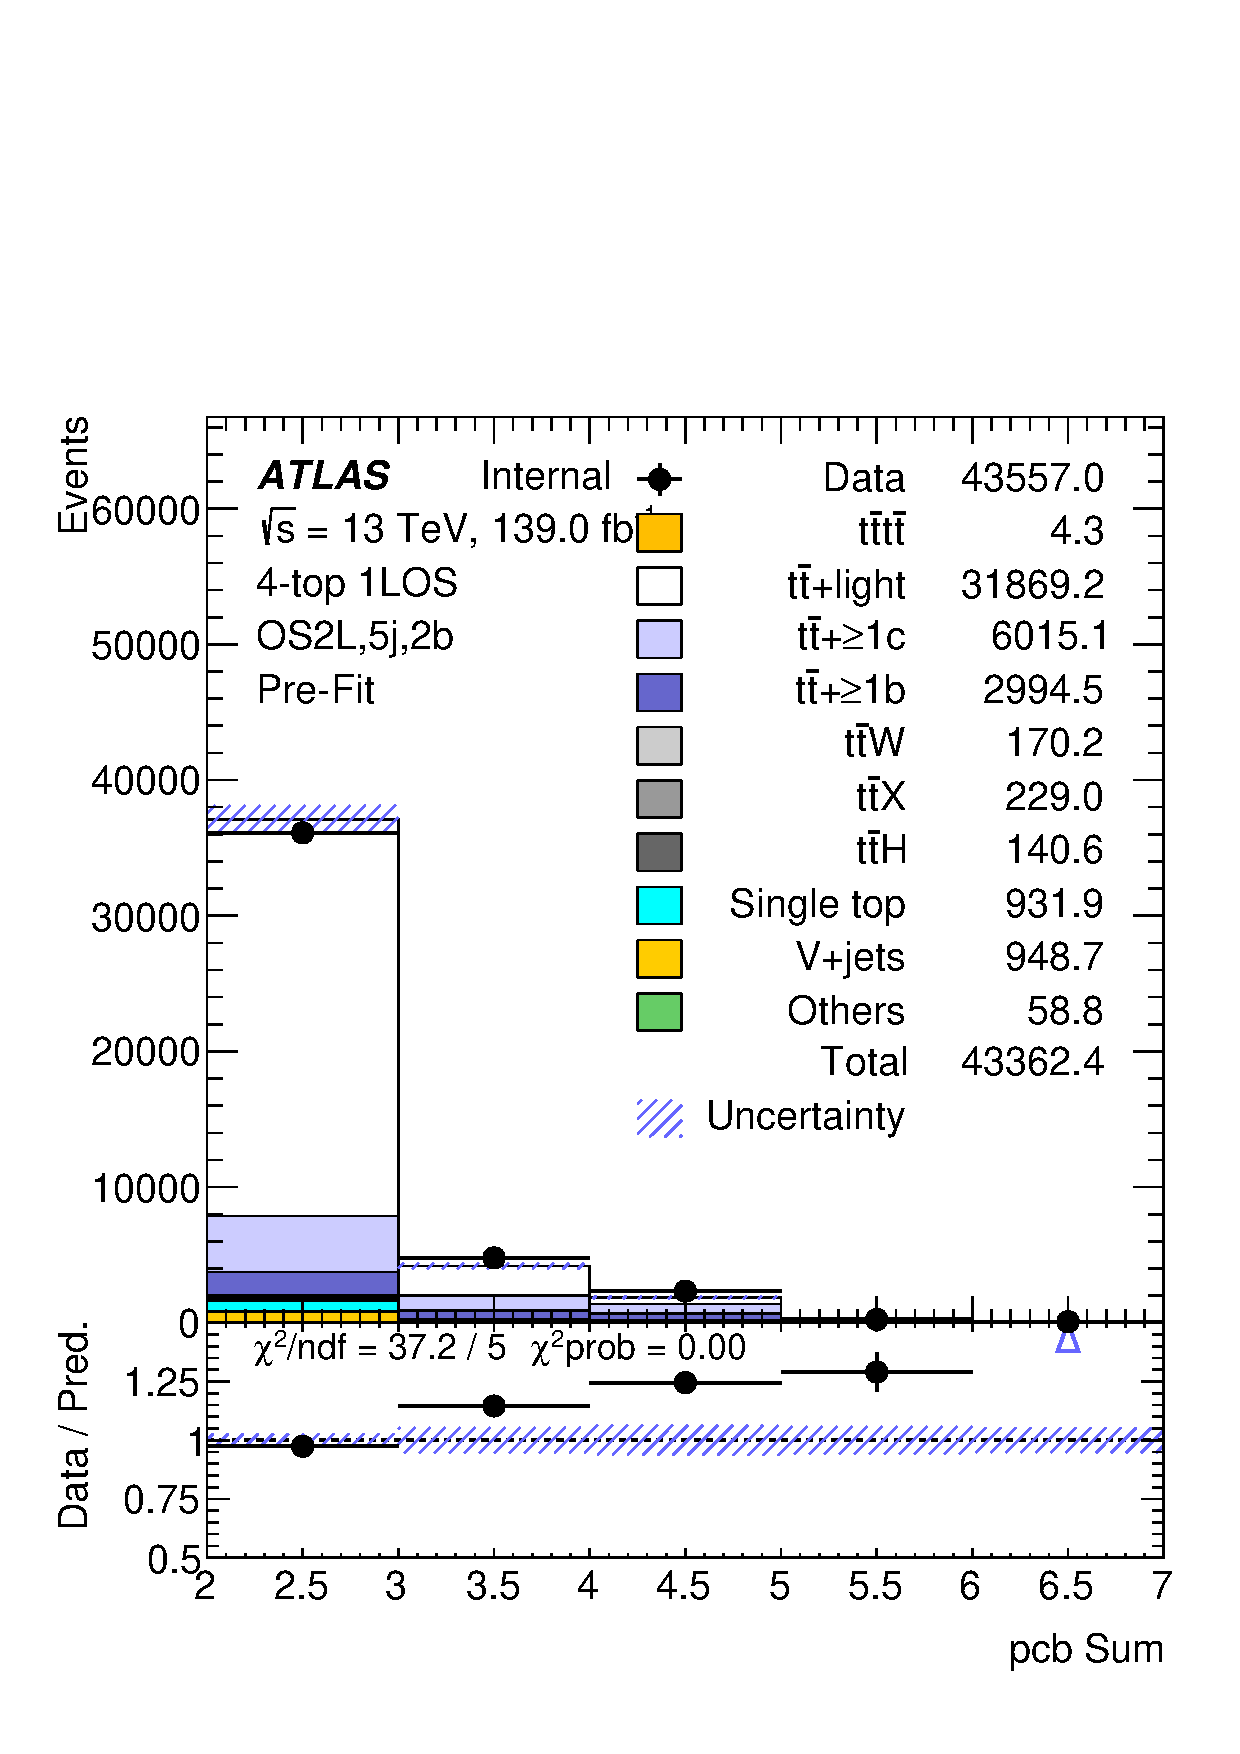
\includegraphics[height=0.28\textheight]{figures/pcbSum34_os2l_5j2b_preFit.pdf}}
  \subfloat[2LOS, $=5j$, $=2b$]{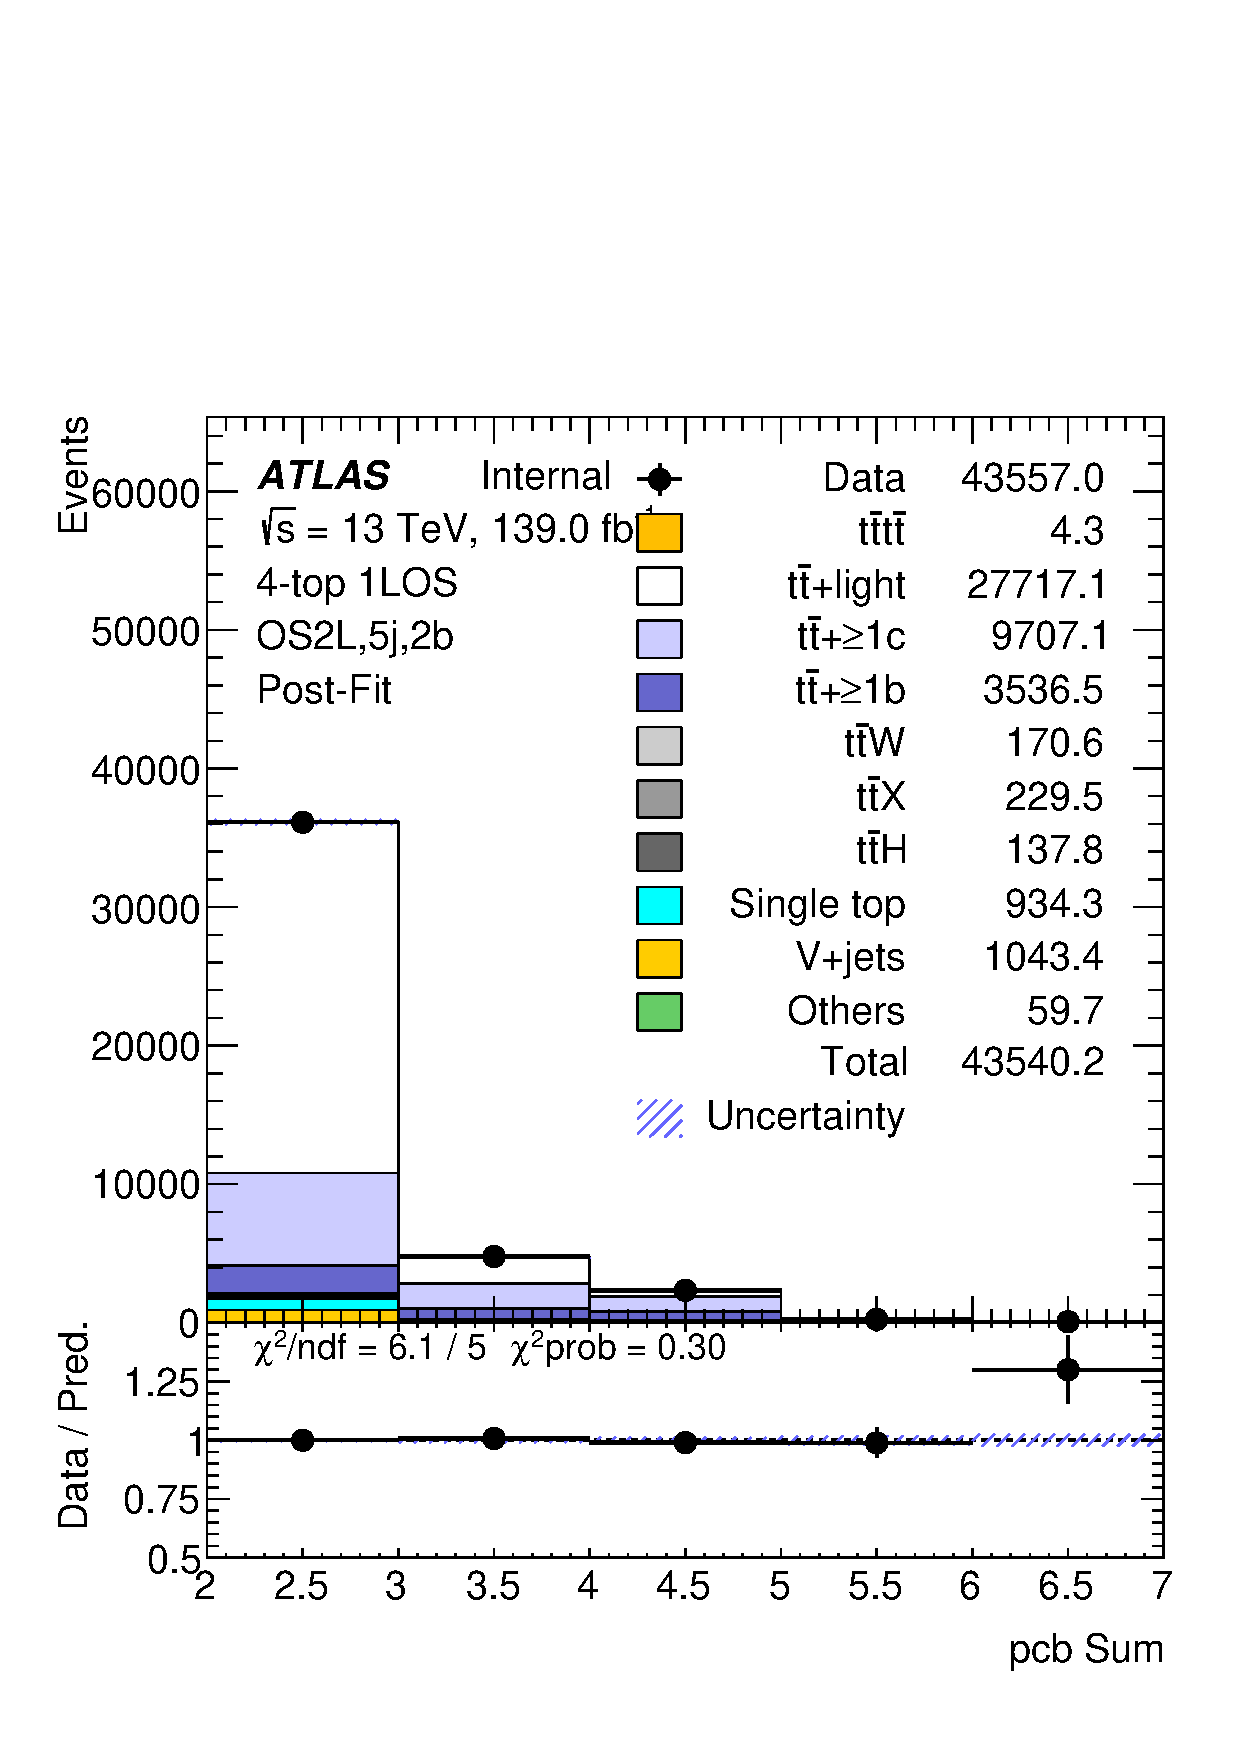
\includegraphics[height=0.28\textheight]{figures/pcbSum34_os2l_5j2b_postFit.pdf}}\\
  \subfloat[2LOS, $=5j$, $=3b$]{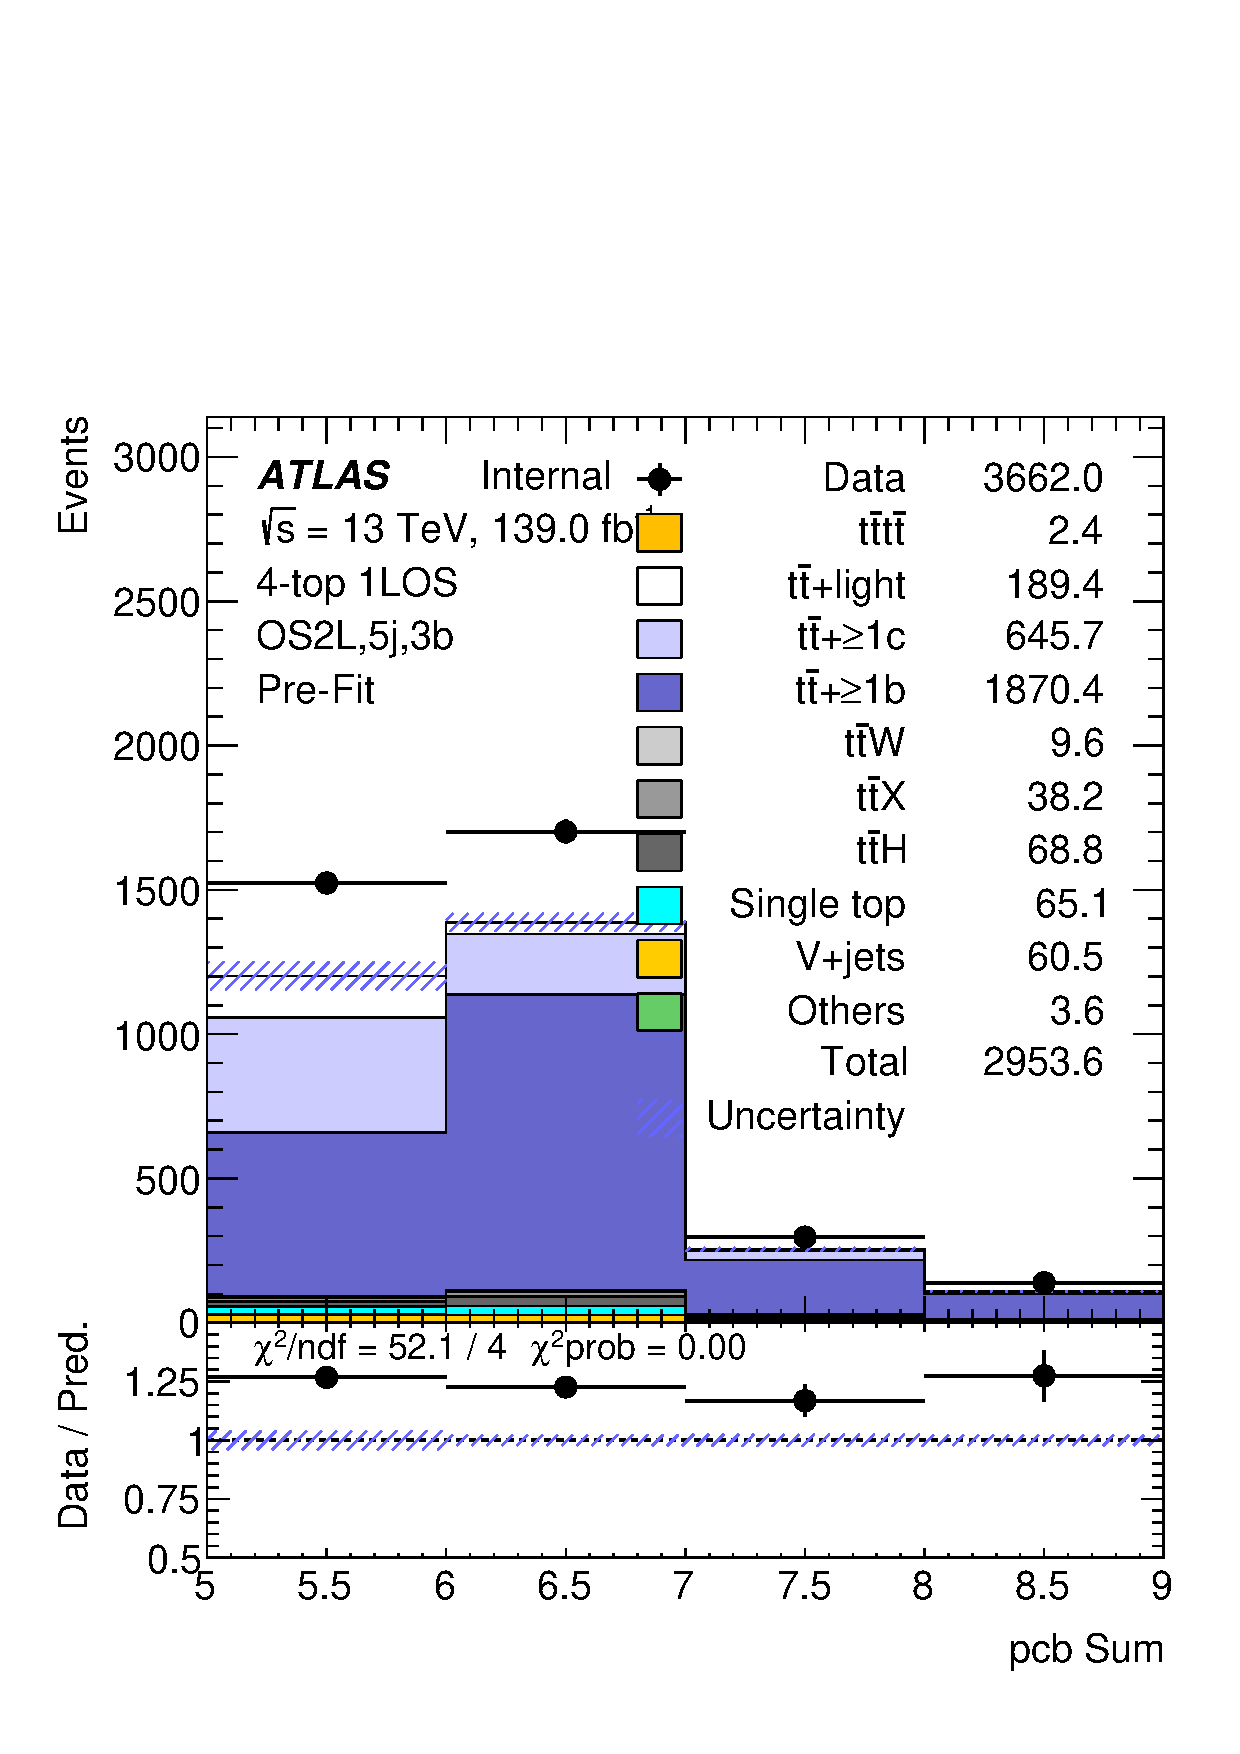
\includegraphics[height=0.28\textheight]{figures/pcbSum34_os2l_5j3b_preFit.pdf}}
  \subfloat[2LOS, $=5j$, $=3b$]{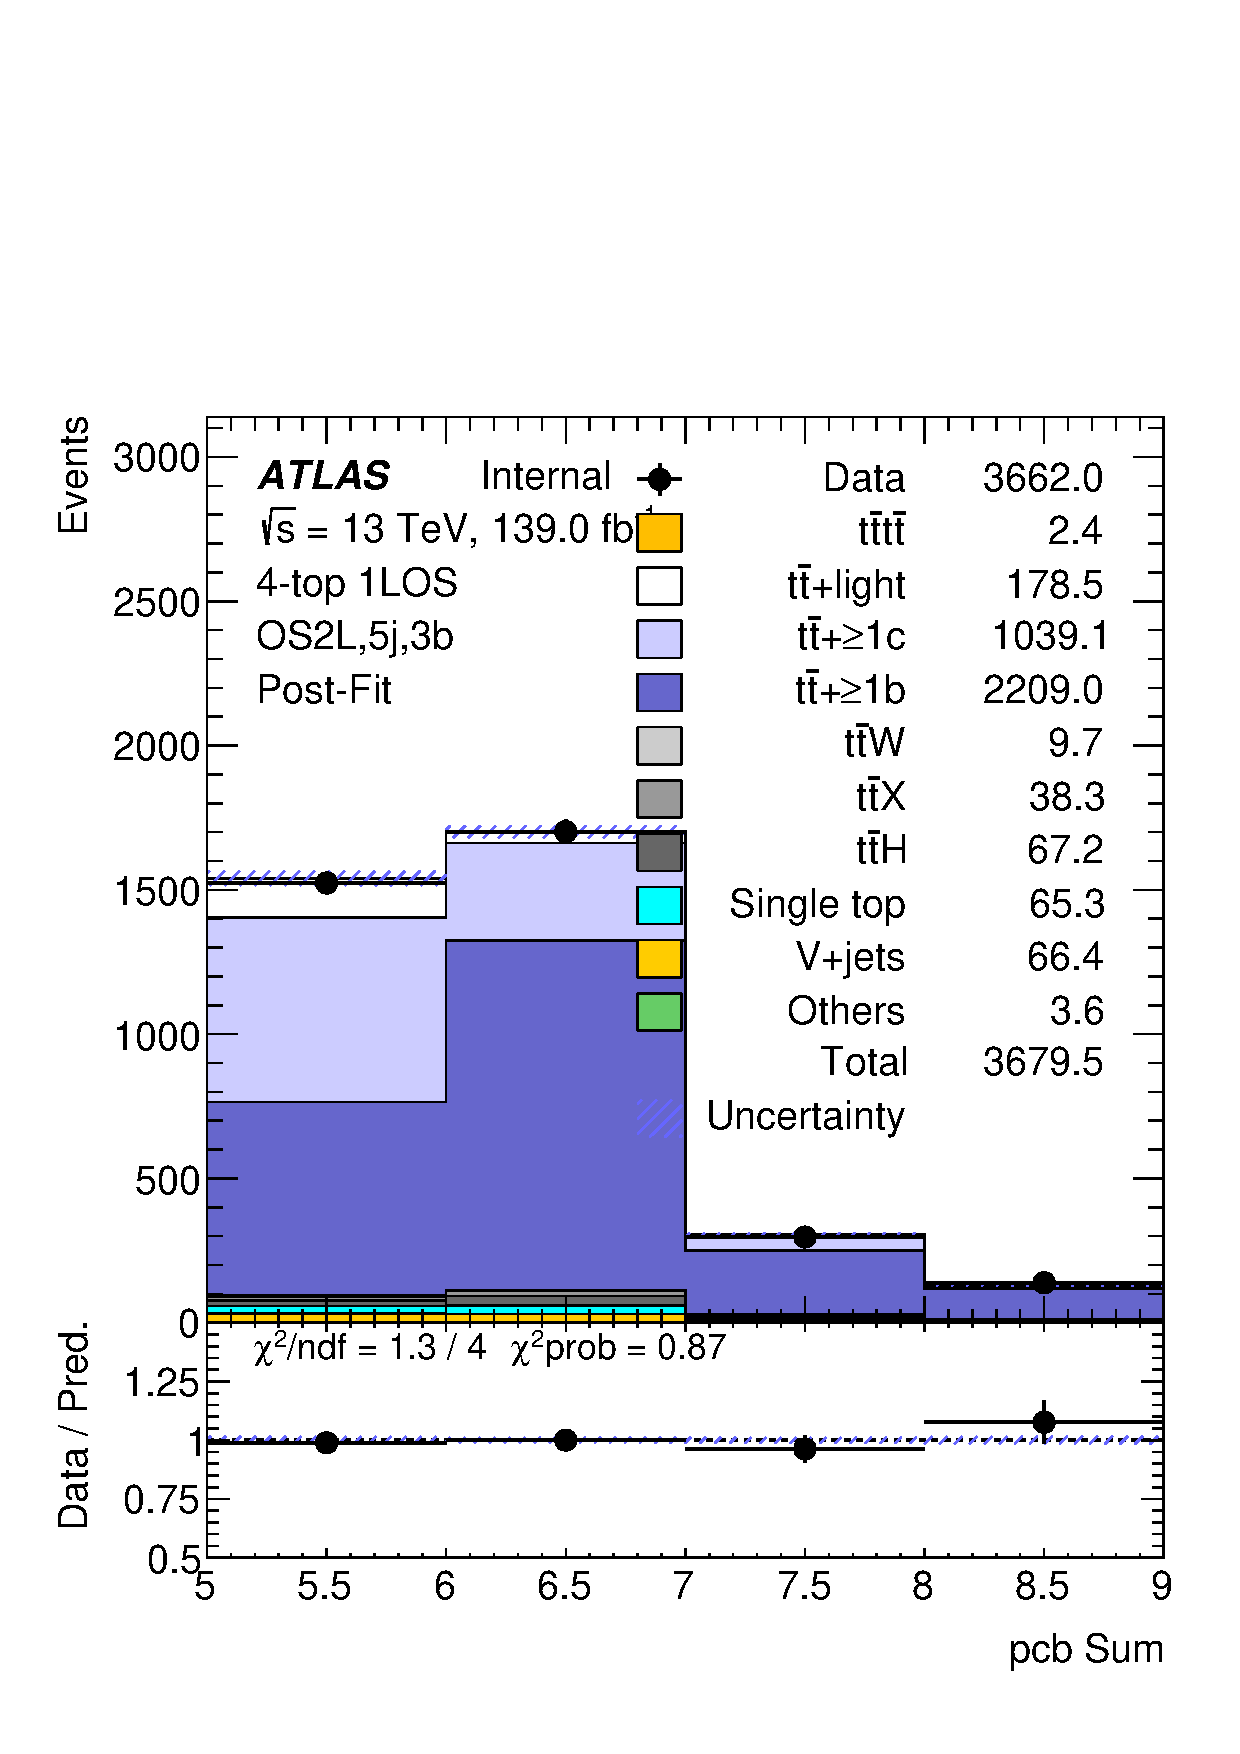
\includegraphics[height=0.28\textheight]{figures/pcbSum34_os2l_5j3b_postFit.pdf}}\\
  \subfloat[2LOS, $=5j$, $\ge4b$]{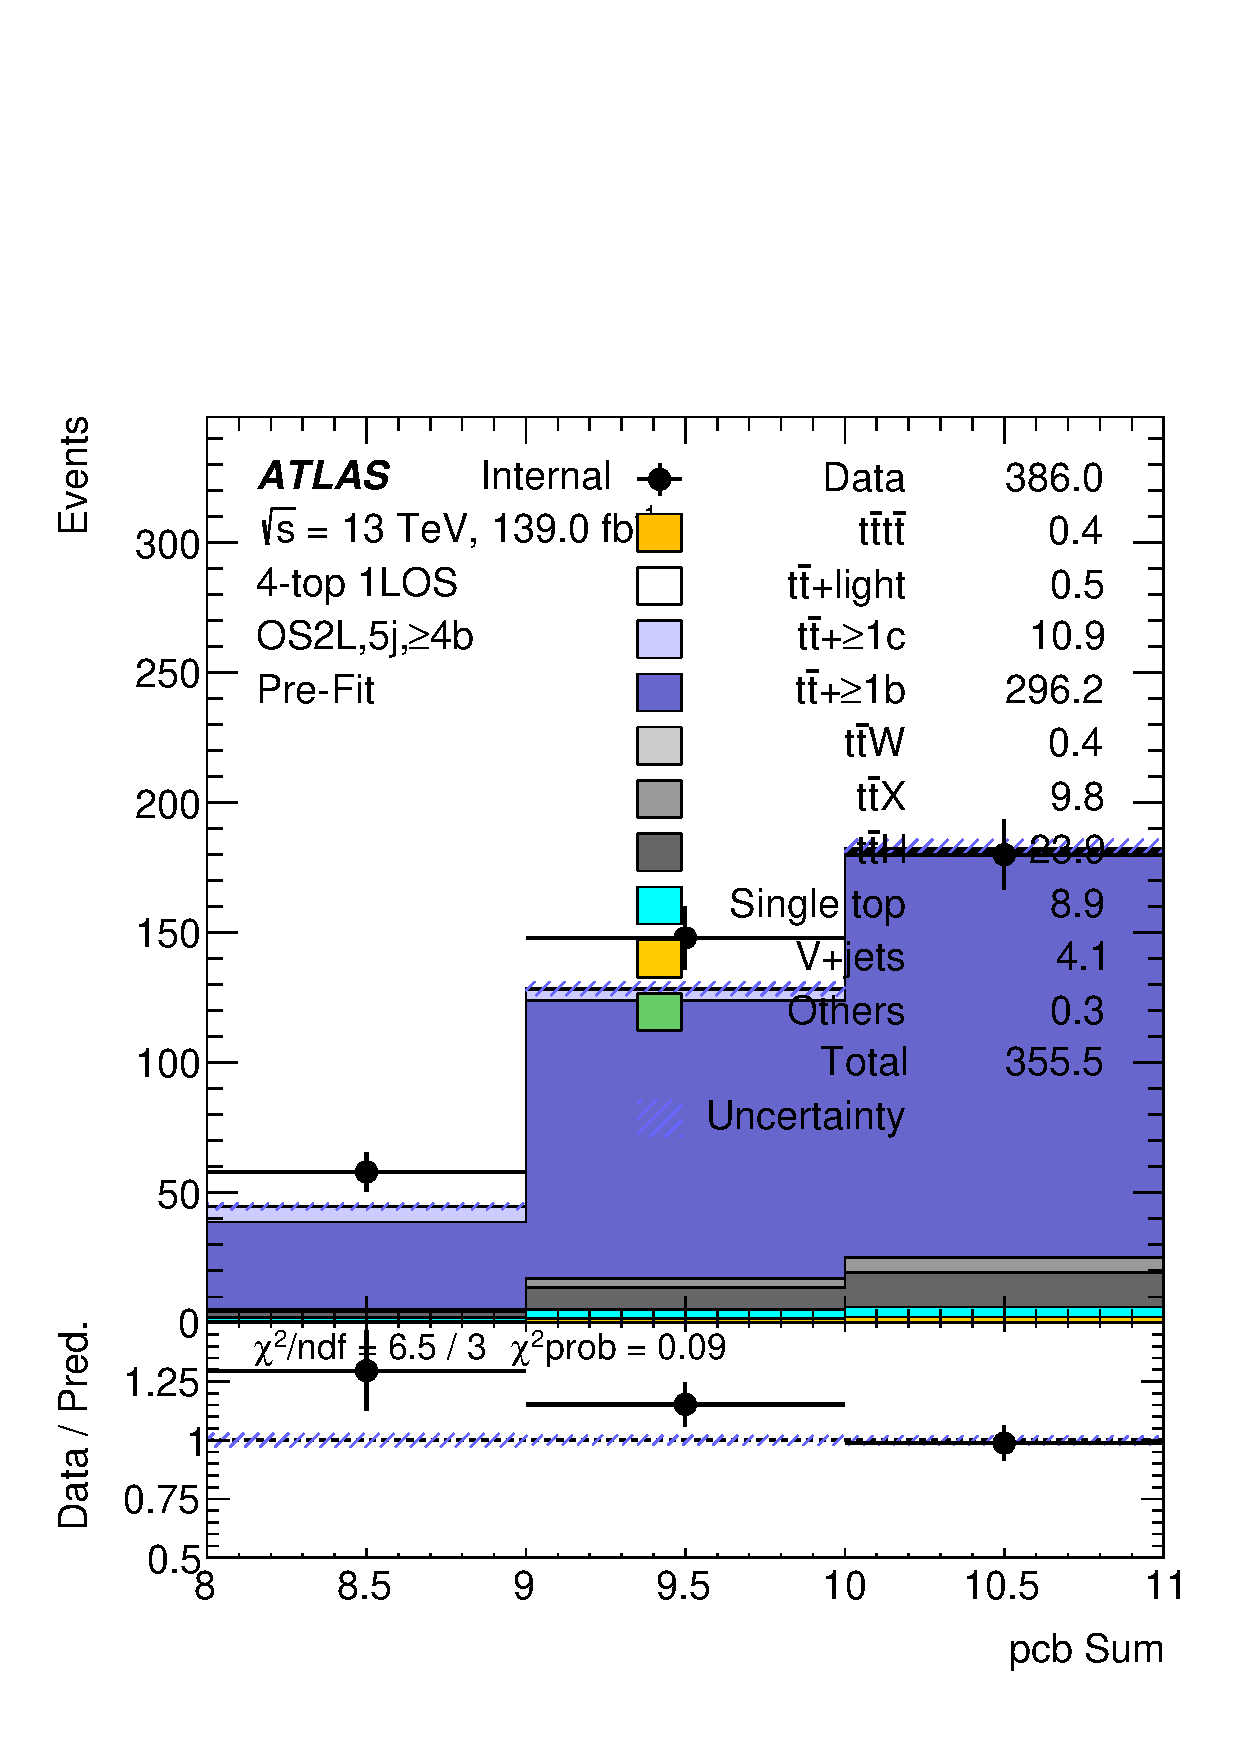
\includegraphics[height=0.28\textheight]{figures/pcbSum34_os2l_5jge4b_preFit.pdf}}
  \subfloat[2LOS, $=5j$, $\ge4b$]{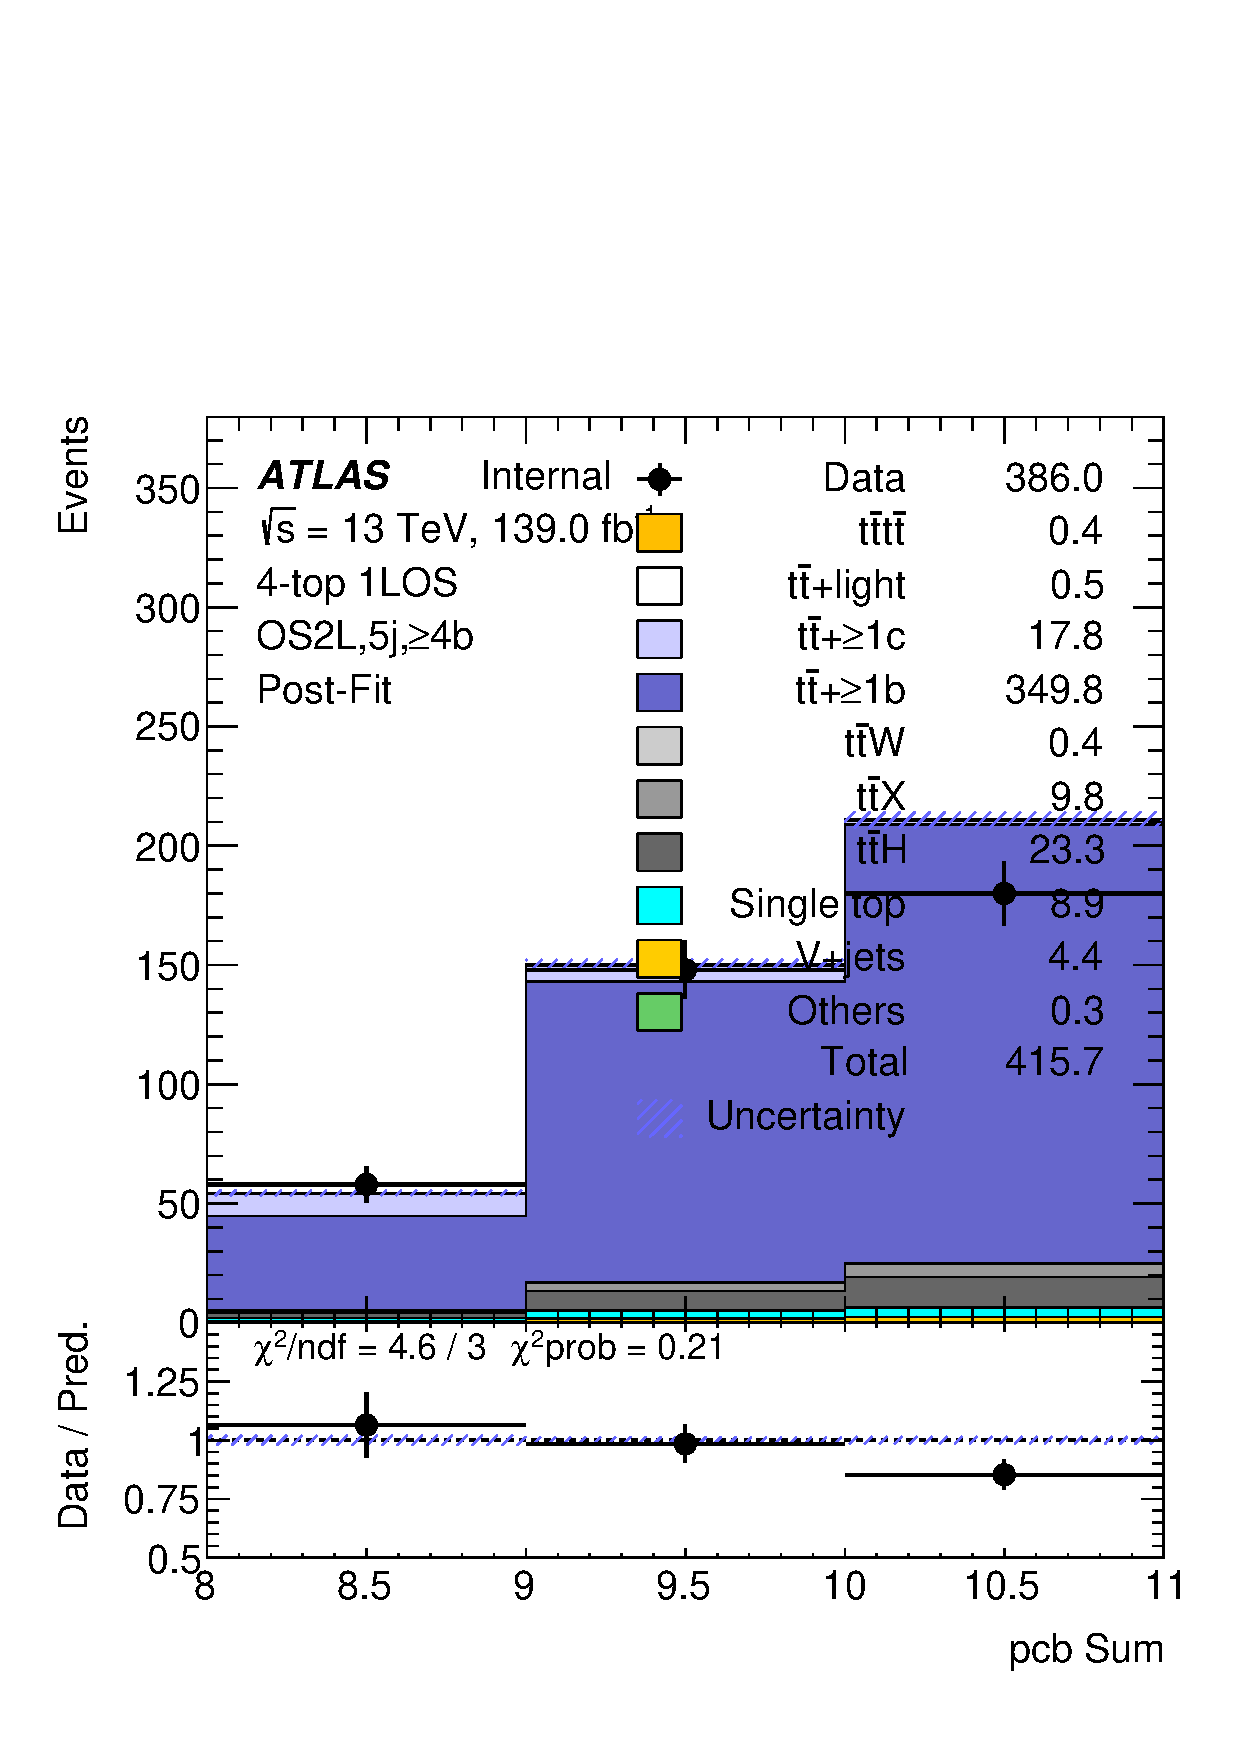
\includegraphics[height=0.28\textheight]{figures/pcbSum34_os2l_5jge4b_postFit.pdf}}
  \caption{Distributions of $\mathrm{pcb}(j_3)+\mathrm{pcb}(j_4)$ in the 2LOS flavour fit regions before (left) and after (right) the fit.}
  \label{fig:2LOS_pcb34_PrePost_thesis}
\end{figure}

\begin{table}[htbp]
  \centering
  \begin{tabular}{lcccc}
    \toprule
      & TTL (1L) & TTL (2LOS) & TTC & TTB \\
    \midrule
    Nominal           & $0.84\pm0.04$ & $0.87\pm0.03$ & $1.61\pm0.13$ & $1.18\pm0.03$ \\
    $t\bar{t}b\bar{b}$ 4FS & $0.83\pm0.04$ & $0.87\pm0.04$ & $1.60\pm0.10$ & $1.17\pm0.02$ \\
    aMC@NLO+Py8       & $0.94\pm0.04$ & $0.96\pm0.04$ & $1.78\pm0.11$ & $1.27\pm0.01$ \\
    Powheg+Herwig     & $0.66\pm0.03$ & $0.73\pm0.03$ & $2.21\pm0.14$ & $1.56\pm0.02$ \\
    \bottomrule
  \end{tabular}
  \caption{Flavour scale factors for the nominal and alternative $t\bar{t}$+jets samples.
  The nominal scale factors are taken from the fit results.
  For alternative samples, scale factors are derived such that the post-fit normalisation of the nominal sample is preserved, ensuring that the flavour correction includes the impact of fitted nuisance parameters.}
  \label{tab:HF_results_thesis}
\end{table}

% Further validation material, including detailed yield tables and channel-by-channel cross-checks, is provided in Appendix~\ref{app:background_modeling_comp}.

\subsection{Multivariate kinematic reweighting}
\label{sec:nn_rew_thesis}

After applying the flavour-dependent normalisation rescaling described above,
residual discrepancies remain between data and simulation in regions
with high jet multiplicity.
These differences primarily affect the jet multiplicity spectrum
and correlated kinematic observables associated with additional QCD radiation.
Given the strong correlations among jet kinematics,
global event variables, and heavy-flavour content,
traditional one-dimensional reweighting techniques are insufficient
to capture the multidimensional structure of the mismodelling.

To address this, a neural-network-based density ratio estimation technique is employed.
Machine learning methods are widely used in high-energy physics
for classification and regression tasks;
however, in the present context the objective is not event classification,
but the estimation of the ratio between probability density functions
describing data and simulation in a multidimensional feature space.
A feed-forward neural network provides a flexible, non-parametric approach
to approximate such density ratios without assuming an explicit functional form.

The training is performed in background-dominated regions
defined by fixed jet multiplicity and exactly two $b$-tagged jets
(1L: $=7j$; 2LOS: $=5j$).
These regions provide a high-purity $t\bar{t}$+jets sample
while maintaining negligible signal contamination.
Separate trainings are carried out for each generator configuration
of the $t\bar{t}$+jets sample in order to preserve the modelling differences
probed by generator systematic variations.

\begin{equation}
  o({\bf x}) = P(\mathrm{data}\,|\,{\bf x}) =
  \frac{\alpha_{\mathrm{data}}\,p_{\mathrm{data}}({\bf x})}
       {\alpha_{\mathrm{data}}\,p_{\mathrm{data}}({\bf x}) + \alpha_{\mathrm{MC}}\,p_{\mathrm{MC}}({\bf x})},
\end{equation}

where $\alpha_{\mathrm{data}}$ and $\alpha_{\mathrm{MC}}$ denote the class proportions used in training.
This expression provides an estimator for the density ratio between data and simulation, which can be translated into an event weight mapping the simulated distribution to that observed in data.

In order to improve stability in limited-statistics regimes, a modified exponential-form objective function is adopted following Ref.~\cite{moustakides2019training}.
With this formulation, the resulting event weight can be expressed as

\begin{equation}
  w({\bf x}) = e^{o({\bf x})}.
\end{equation}

The training is performed in background-dominated regions defined by fixed jet multiplicity and exactly two $b$-tagged jets (1L: $=7j$; 2LOS: $=5j$).
These regions provide a high-purity $t\bar{t}$+jets sample while maintaining negligible signal contamination.
Separate trainings are carried out for each generator configuration of the $t\bar{t}$+jets sample to preserve the modelling differences probed by generator systematics.

The input features include the multiplicity and kinematics of reconstructed jets and re-clustered jets, missing transverse momentum, and the leading lepton kinematics.
Non-$t\bar{t}$ contributions are effectively subtracted by including them in the training with a data label and negative event weights, such that the learned density ratio targets the $t\bar{t}$+jets component only.

The derived reweighting improves the agreement between data and simulation not only for the input observables but also for derived quantities, demonstrating that correlations are correctly captured.
An illustration of the impact on the $H_T$ distribution in the 1L channel is shown in Figure~\ref{fig:cor1l_thesis}.
By construction, the reweighting procedure is shape-only; the stability of the overall normalisation after reweighting is verified explicitly.

\begin{figure}[htbp]
  \centering
  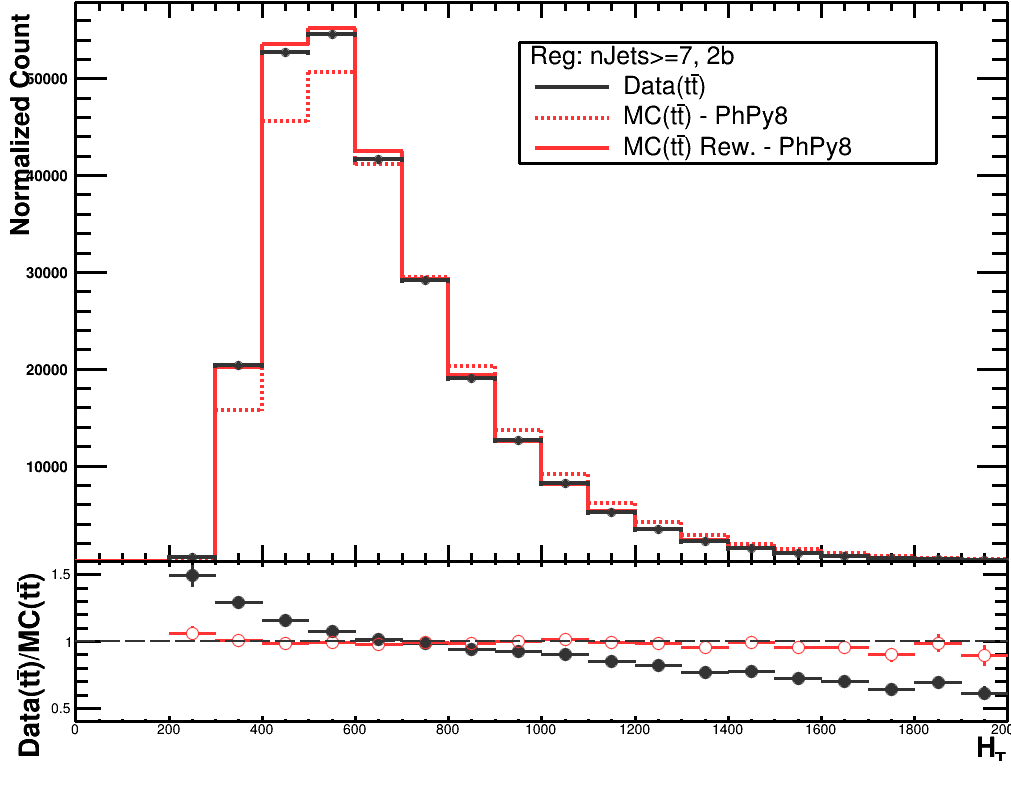
\includegraphics[width=0.48\textwidth]{figures/cor_1l_nom.png}
  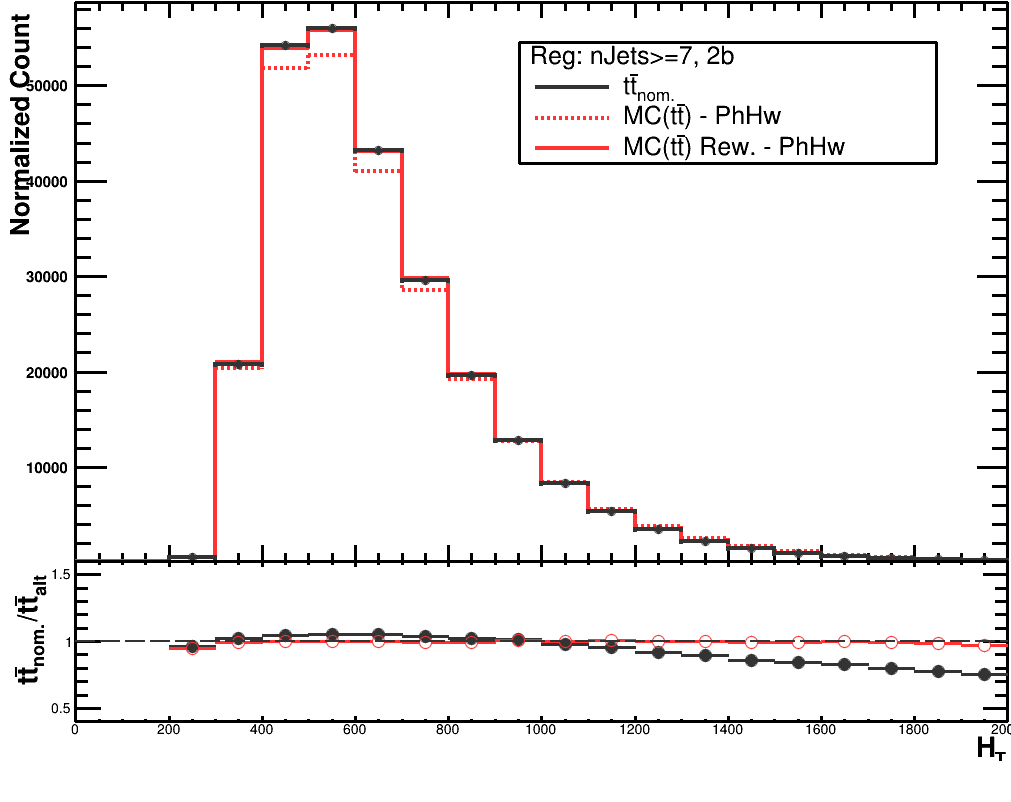
\includegraphics[width=0.48\textwidth]{figures/cor_1l_alt.png}
  \caption{Illustration of the multivariate kinematic reweighting for $H_T$ in the 1L channel, shown for the nominal $t\bar{t}$+jets sample (left) and an alternative generator configuration (right).
  The ratio panels compare data to $t\bar{t}$+jets prediction after heavy-flavour rescaling (black) and after applying both the flavour and kinematic corrections (red).}
  \label{fig:cor1l_thesis}
\end{figure}

\subsubsection{Uncertainty treatment for data-driven corrections}
\label{sec:NN_reweighting_unc_thesis}

Two dedicated uncertainties are introduced to propagate the impact of the data-driven corrections to the final likelihood fit.

First, the kinematic reweighting depends on the subtraction of non-$t\bar{t}$ processes from data in the training region.
To account for this, the normalisation of non-$t\bar{t}$ backgrounds entering the subtraction is varied by $\pm 50\%$, and alternative weights are derived.
The resulting shape difference is propagated as a nuisance parameter in the signal extraction fit, with an impact of typically 3--4\% on the fitted distributions.

Second, statistical limitations in the training data and simulation introduce an uncertainty on the learned reweighting function.
This effect is evaluated using the MC dropout technique~\cite{gal2016dropout}, where dropout layers are kept active at inference time and the network is evaluated repeatedly to obtain an ensemble of weights.
The standard deviation of the resulting variations is used to define a shape uncertainty, propagated as a nuisance parameter in the likelihood fit.
% Validation studies on toy models and representative analysis regions are documented in Appendix~\ref{app:NNRewPlots}.

\subsection{Summary}
\label{sec:ttjets_modelling_summary}

In summary, a two-step data-driven correction strategy is applied to the $t\bar{t}$+jets background prior to the signal extraction.
A flavour-dependent normalisation rescaling corrects the flavour composition
of the $t\bar{t}$+jets background using $b$-tagging-sensitive control regions,
while a multivariate neural-network-based reweighting corrects correlated mismodelling in jet multiplicity and kinematics.
Both corrections are propagated to the final likelihood fit with dedicated nuisance parameters accounting for subtraction and statistical effects.

Figure~\ref{fig:effect_data_driven_corr} illustrates the impact of the combined corrections in inclusive regions containing all control, validation and signal regions.
Distributions of key observables relevant for the analysis sensitivity, such as $H_T$, jet multiplicity, and the multiplicity of re-clustered jets,
are shown for the 1L and 2LOS channels.
A significant improvement in the agreement between data and the background prediction is observed both in the overall normalisation and in the shape of the distributions.
These corrections therefore provide a more reliable modelling of the dominant $t\bar{t}$+jets background across the phase space relevant for the signal extraction.

\begin{figure}[]
  \centering
  \subfloat[]{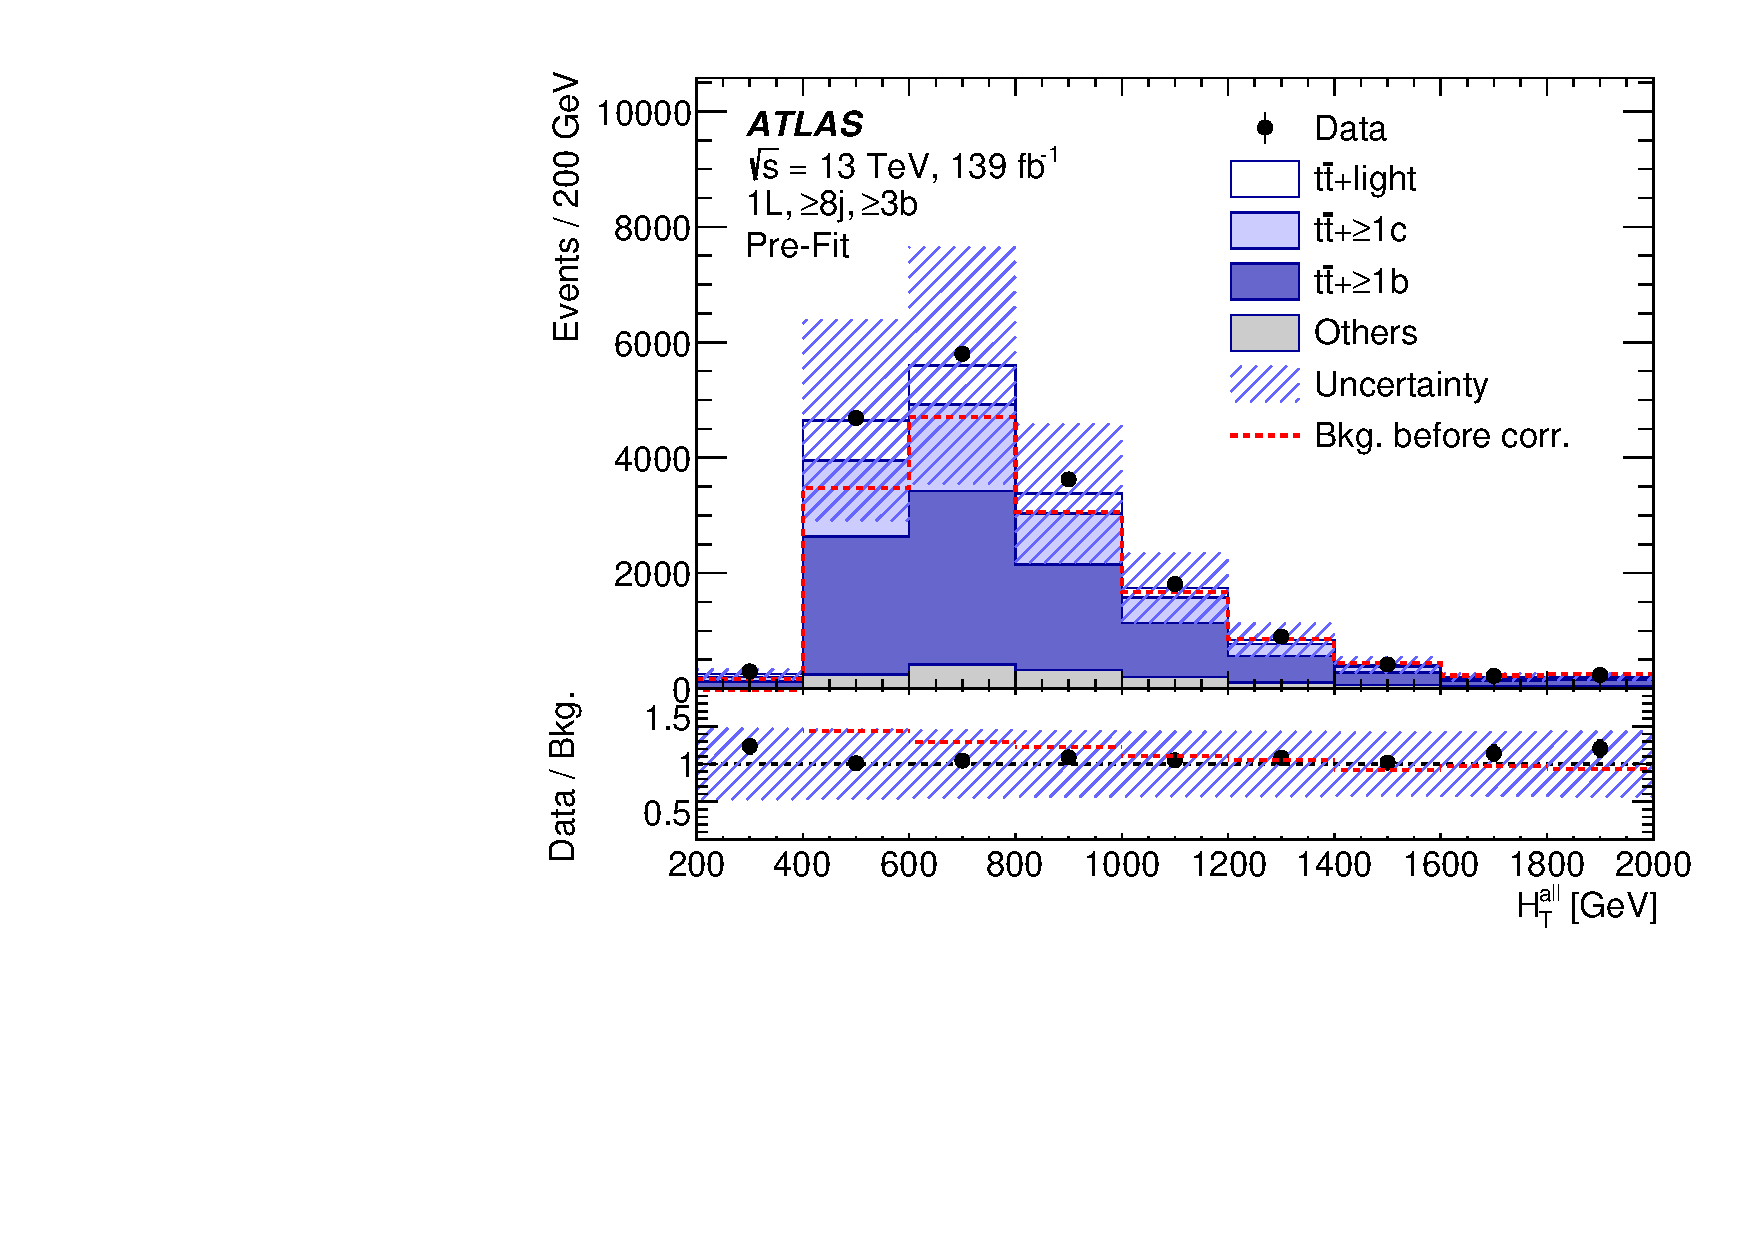
\includegraphics[width=0.495\textwidth]{figures/figures_paper/val_ljets_ge8jge3b_HT_all.pdf}}
  \subfloat[]{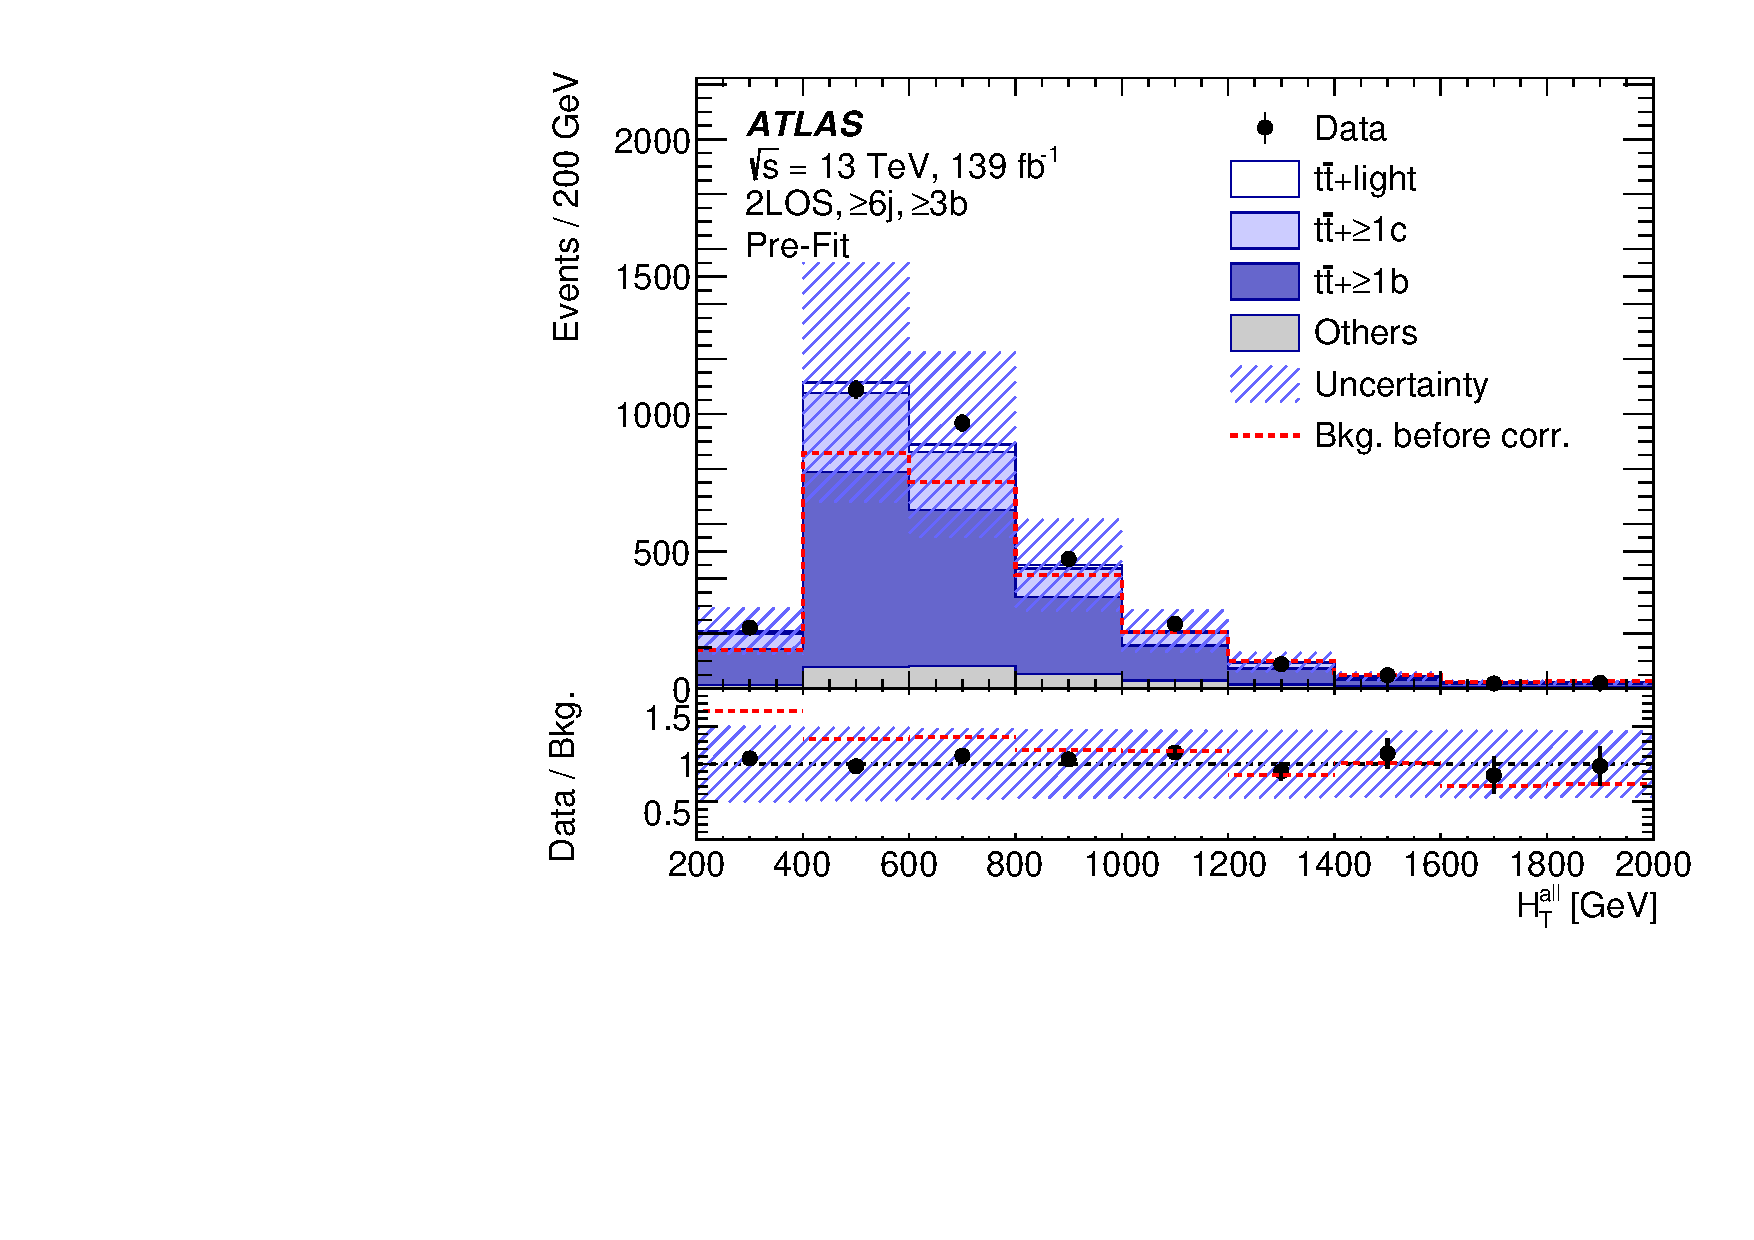
\includegraphics[width=0.495\textwidth]{figures/figures_paper/val_os2l_ge6jge3b_HT_all.pdf}}\\
  \subfloat[]{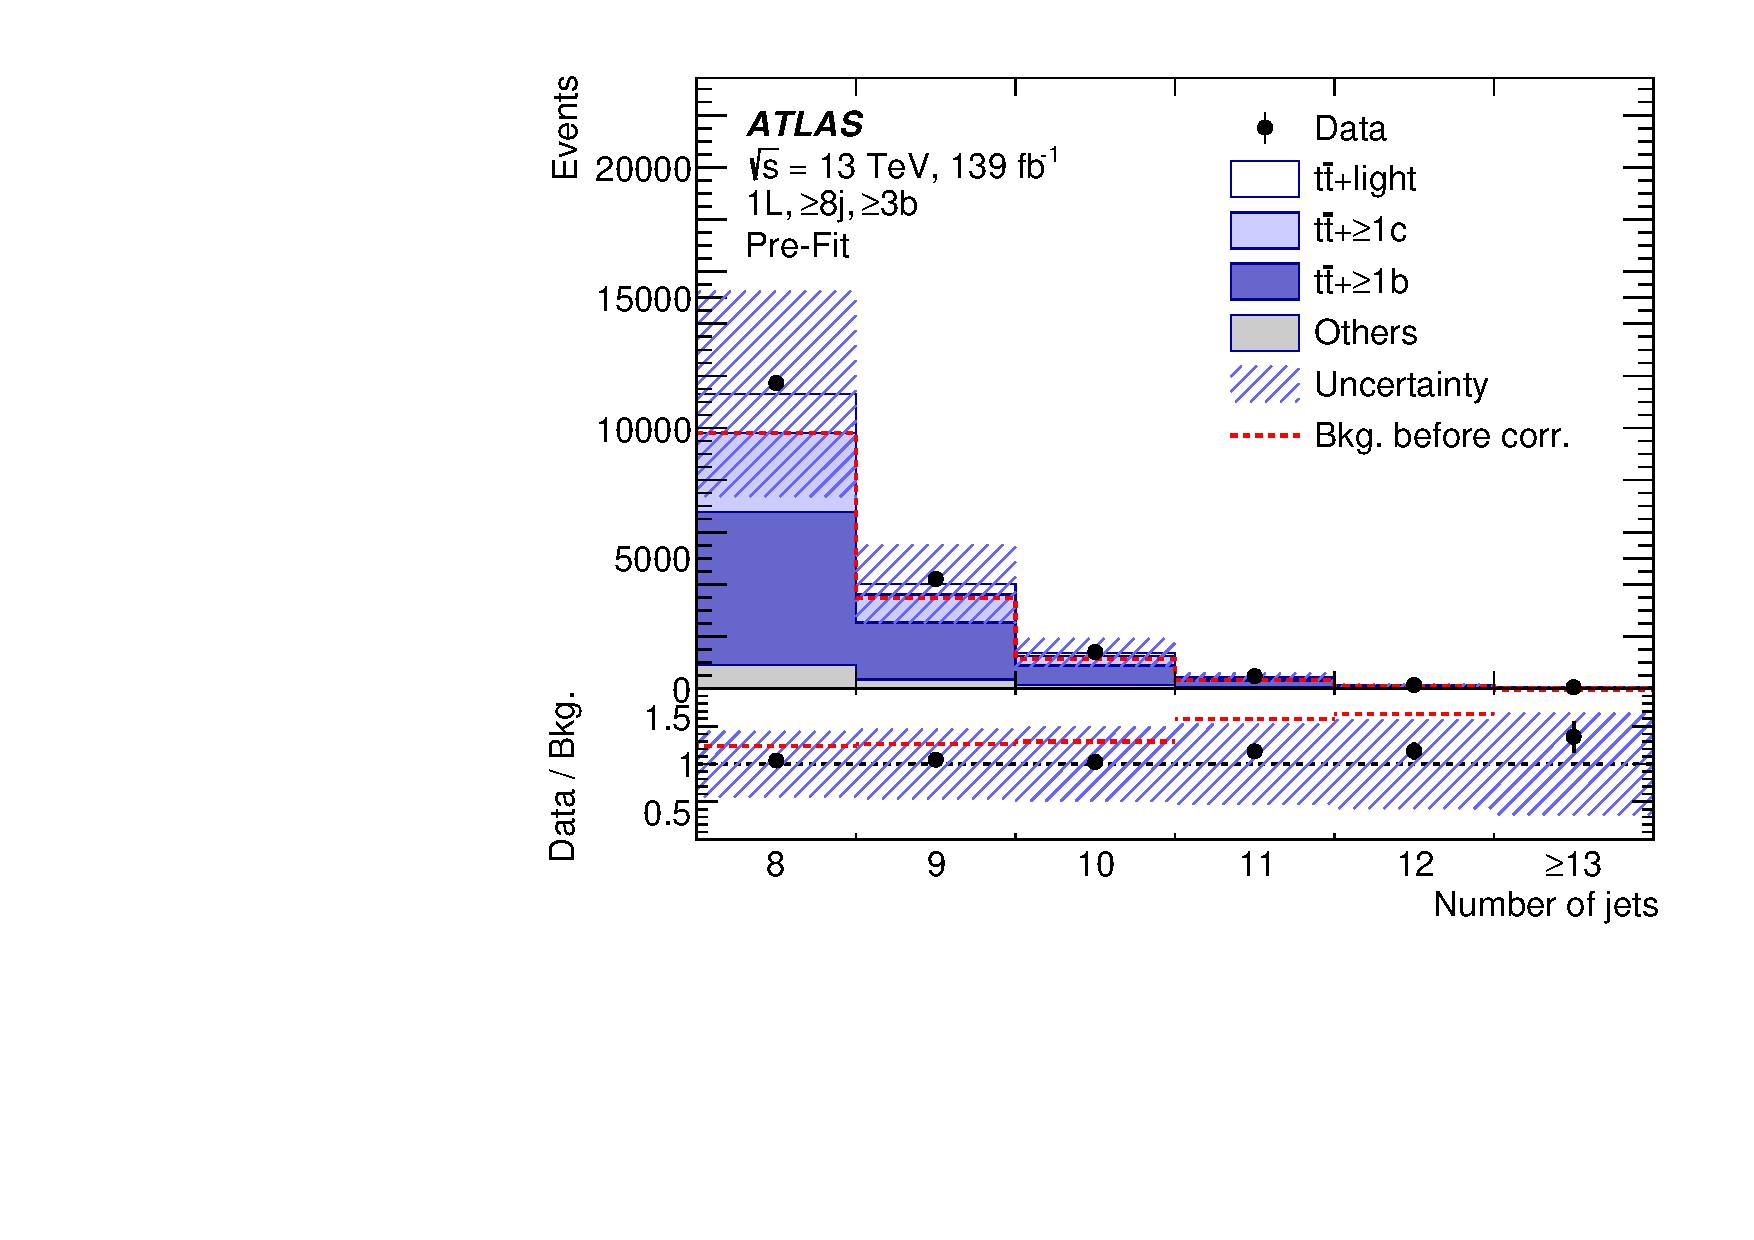
\includegraphics[width=0.495\textwidth]{figures/figures_paper/val_ljets_ge8jge3b_nJets.pdf}}
  \subfloat[]{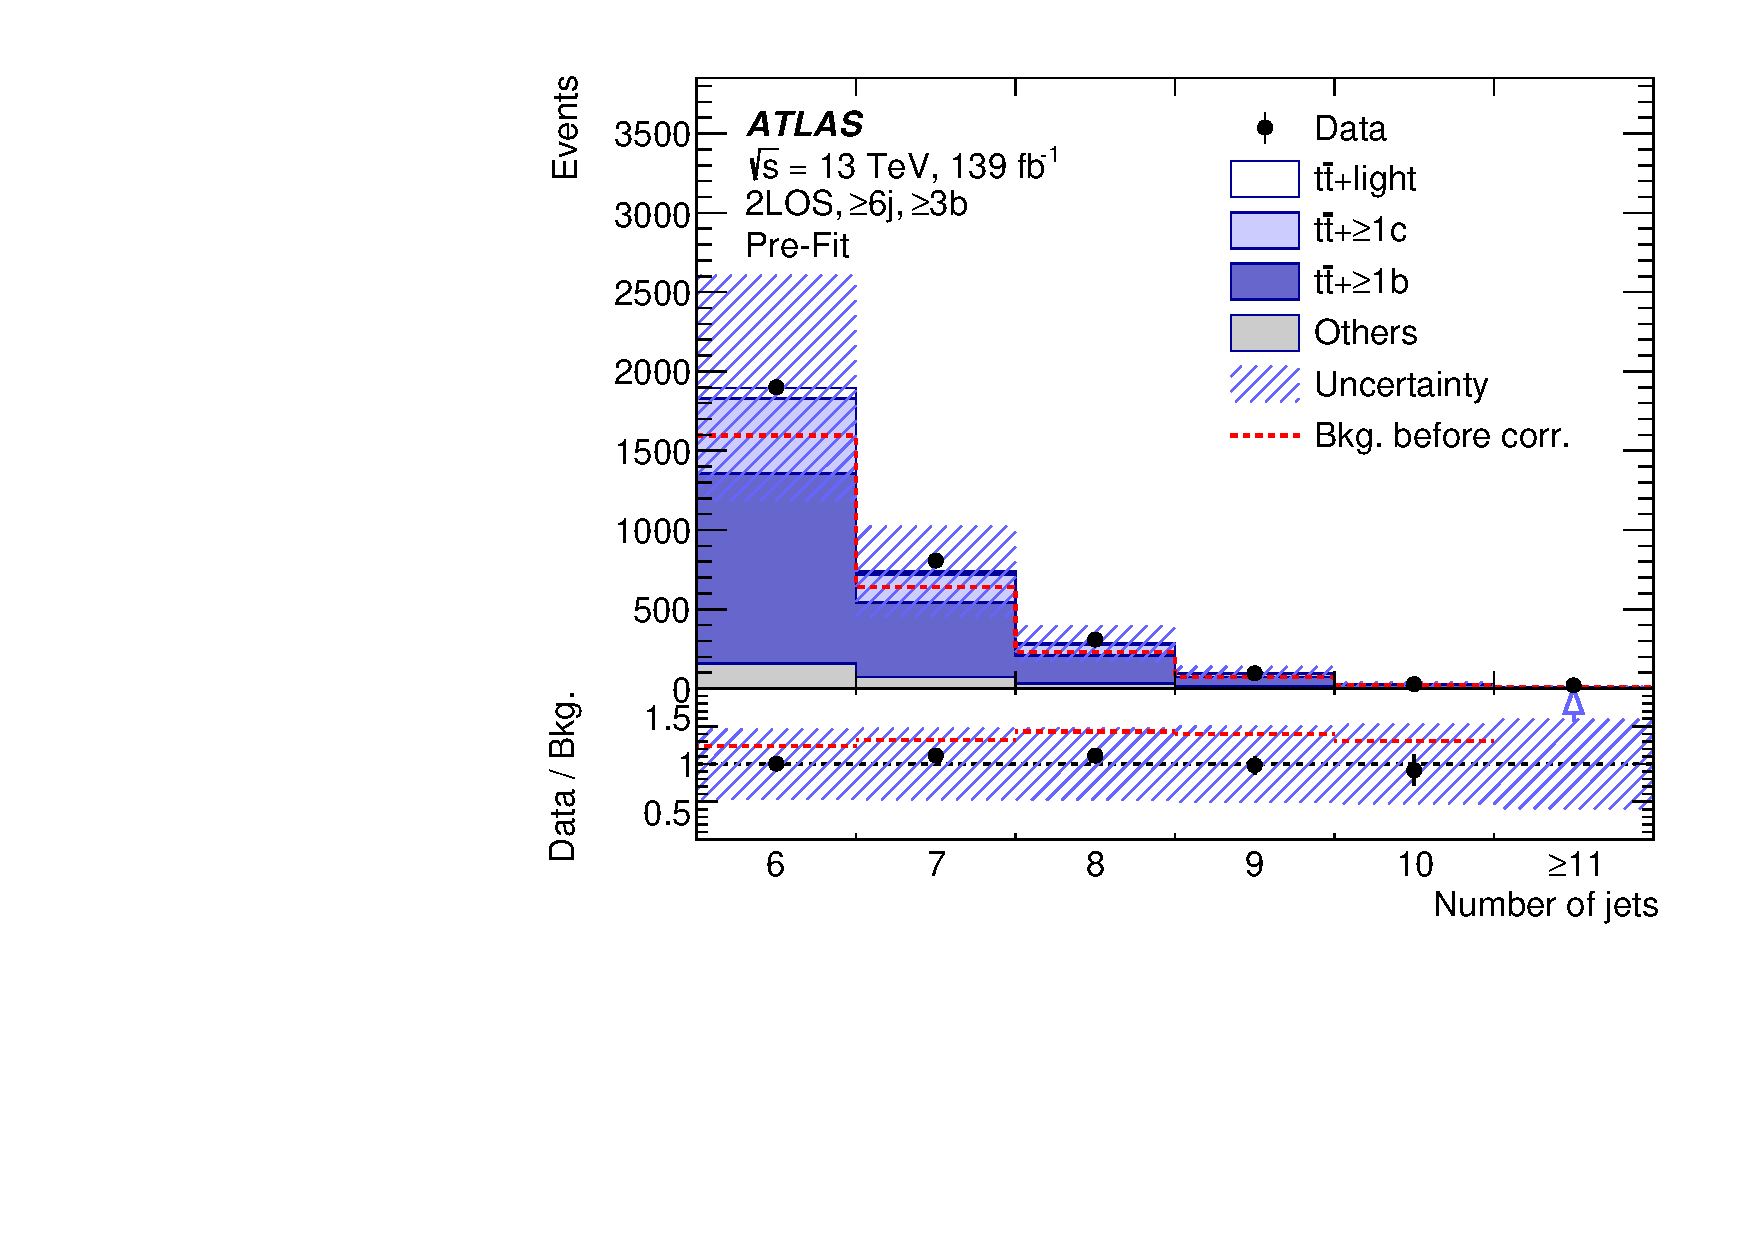
\includegraphics[width=0.495\textwidth]{figures/figures_paper/val_os2l_ge6jge3b_nJets.pdf}}\\
  \subfloat[]{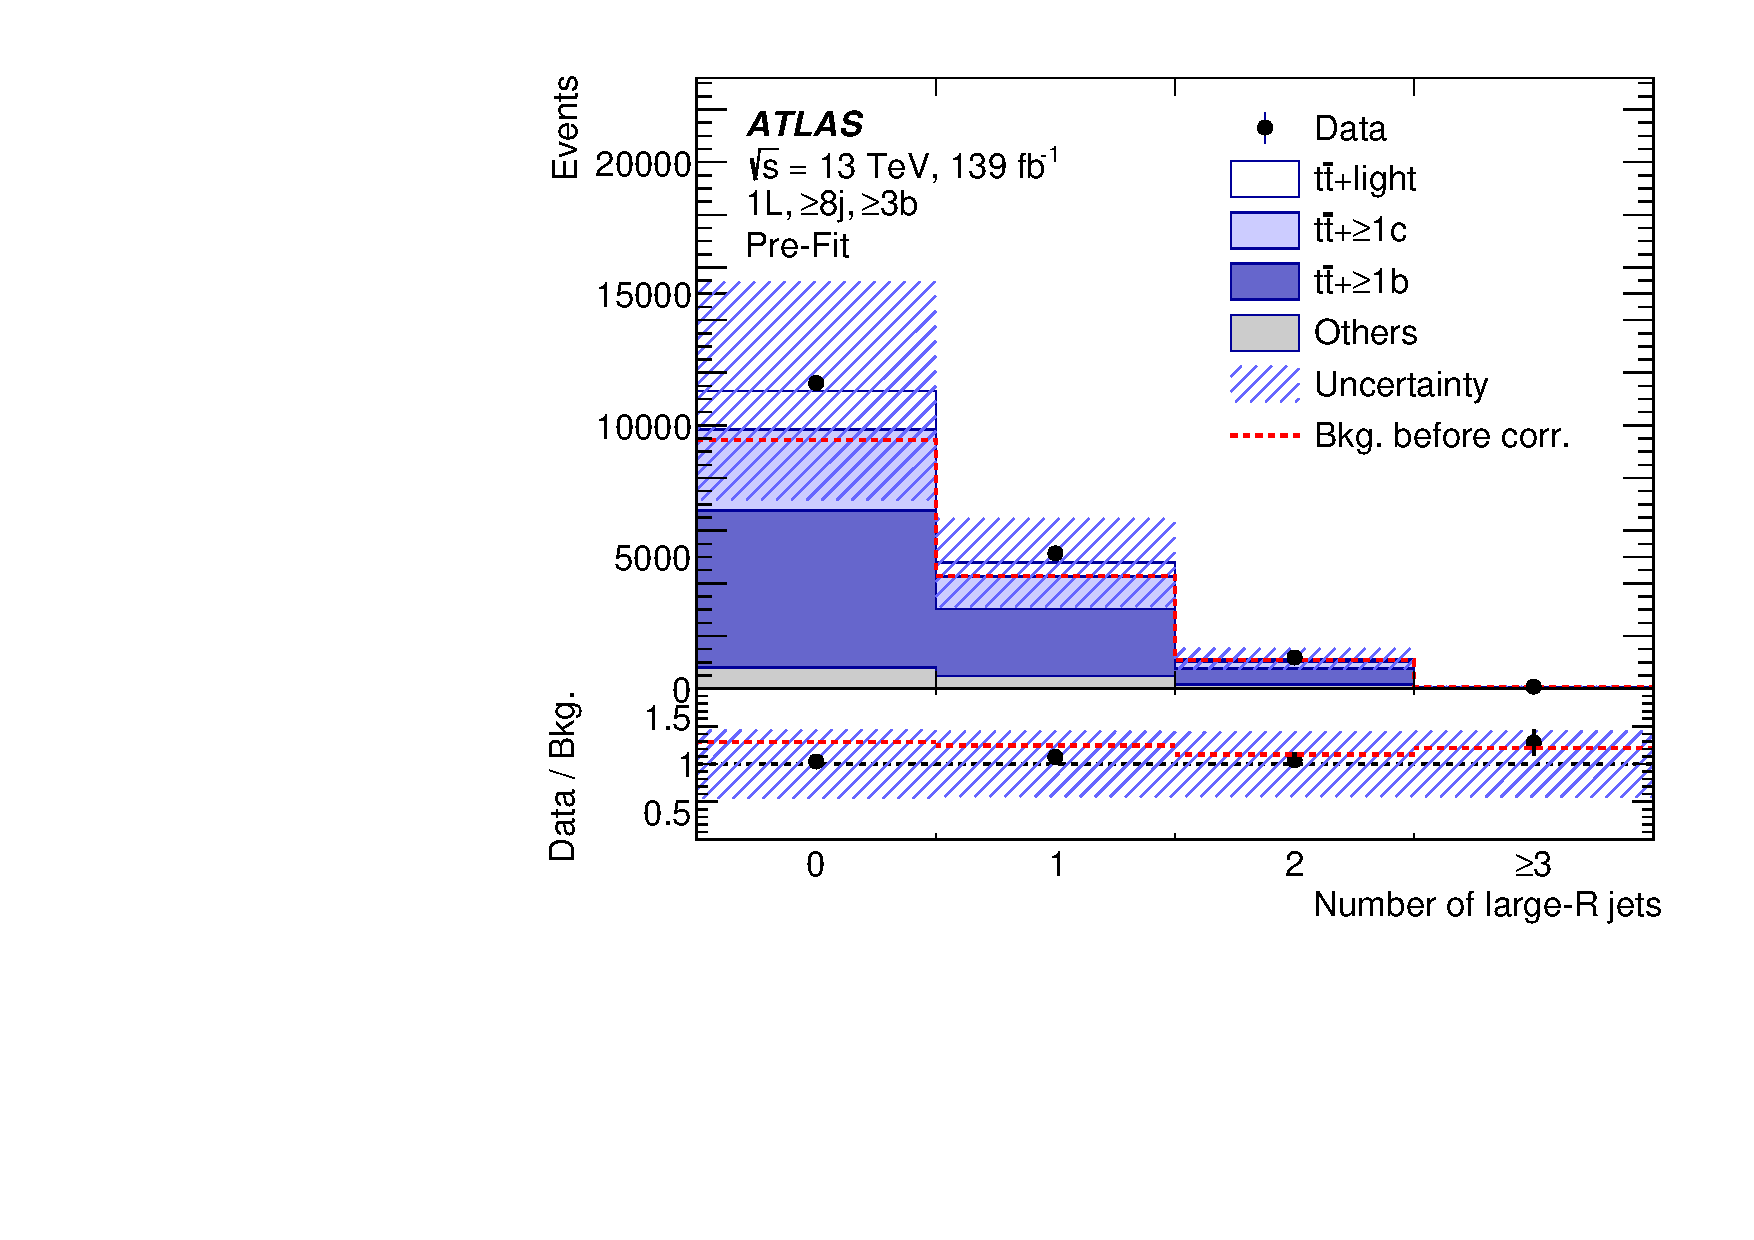
\includegraphics[width=0.495\textwidth]{figures/figures_paper/val_ljets_ge8jge3b_nRCJetsM100.pdf}}
  \subfloat[]{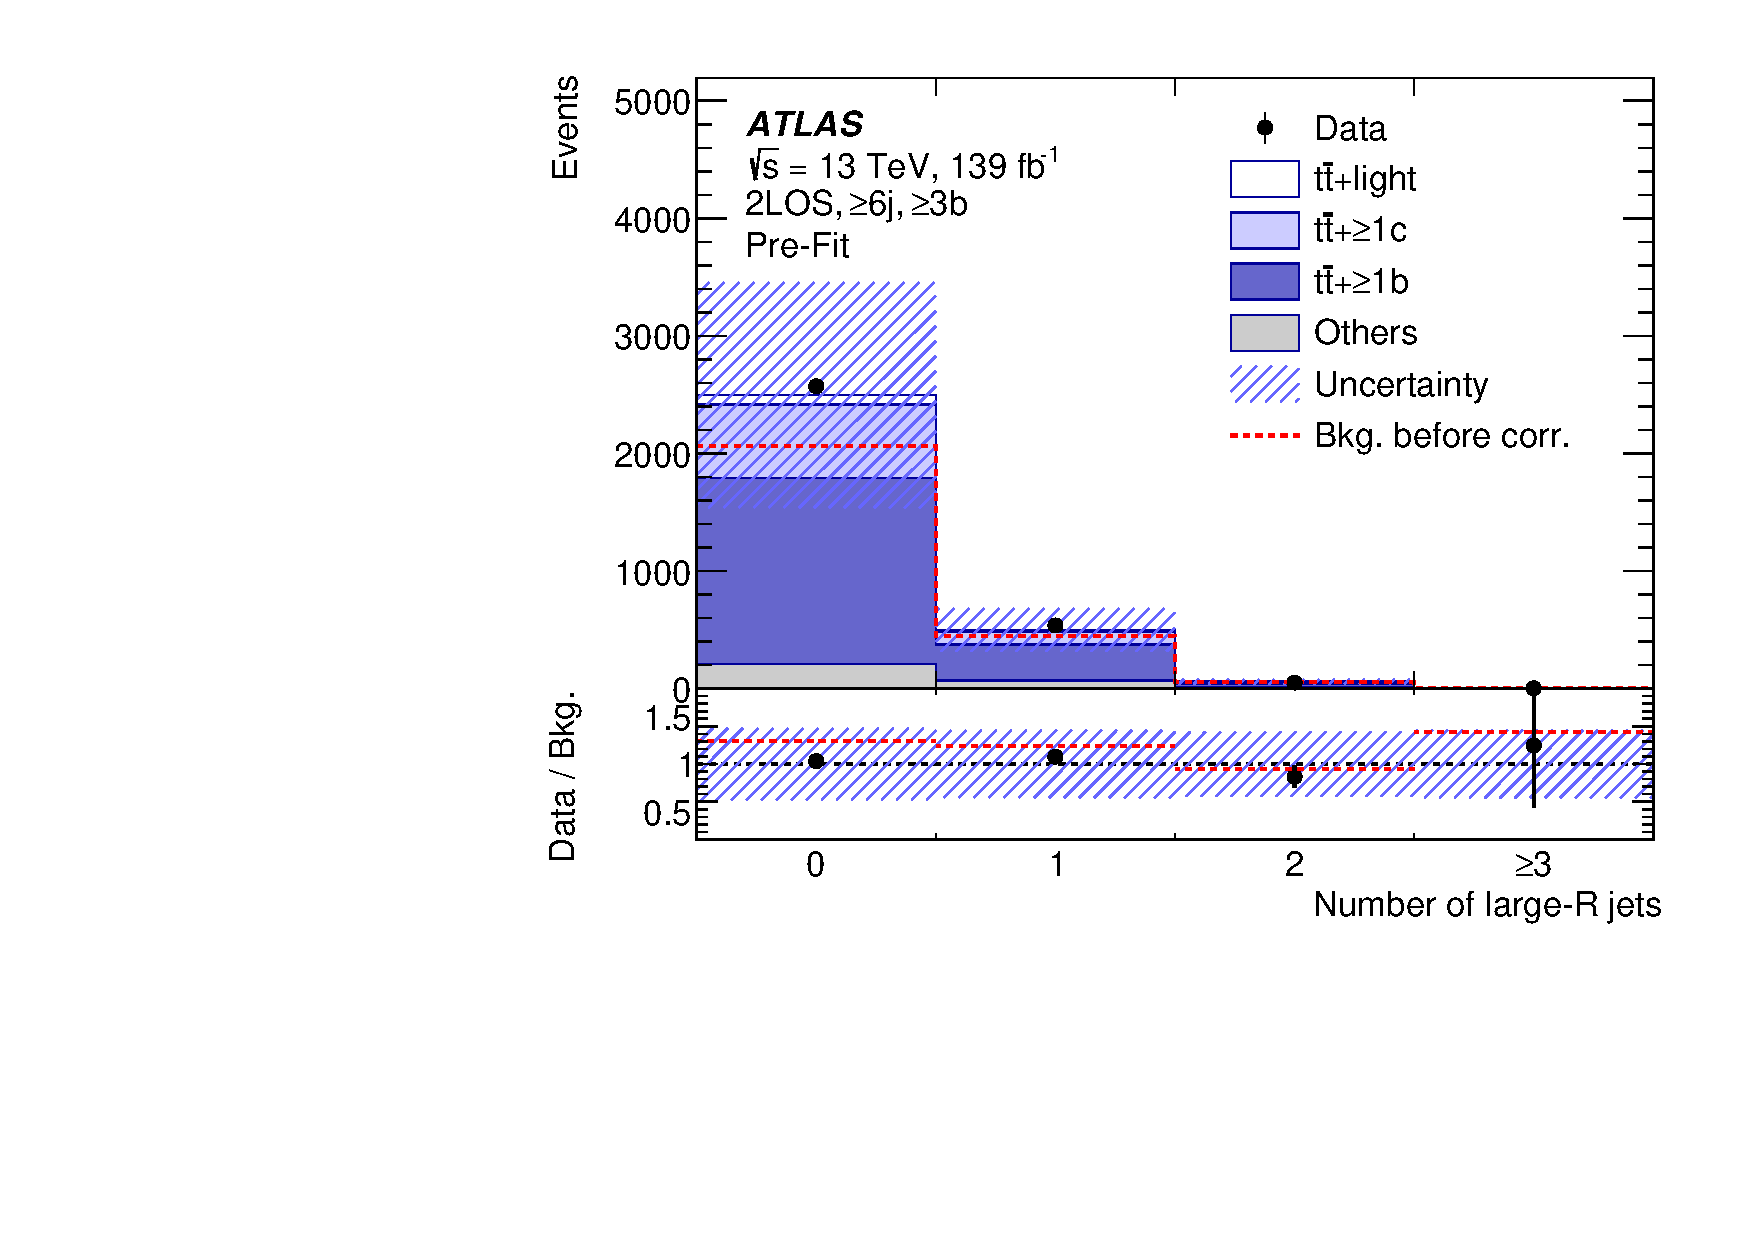
\includegraphics[width=0.495\textwidth]{figures/figures_paper/val_os2l_ge6jge3b_nRCJetsM100.pdf}}
  \caption{
    The comparison of (a, b) $H_{\mathrm{T}}$, (c, d) $N_{\mathrm{jets}}$ and (e, f) $N_{\mathrm{large}R\text{-jets}}$ distributions
    between data and background predictions before and after applying the data-driven corrections,
    shown separately for the 1L and 2LOS channels.
    The corrected prediction is shown as coloured stacks,
    while the prediction before applying the corrections is indicated by the red dashed line.
    The hashed band represents the total uncertainty in the background prediction.
    The last bin in each distribution contains the overflow.}
  \label{fig:effect_data_driven_corr}
\end{figure}